% Options for packages loaded elsewhere
\PassOptionsToPackage{unicode}{hyperref}
\PassOptionsToPackage{hyphens}{url}
\PassOptionsToPackage{dvipsnames,svgnames,x11names}{xcolor}
%
\documentclass[
  11pt,
  a4paper,
]{report}

\usepackage{amsmath,amssymb}
\usepackage{setspace}
\usepackage{iftex}
\ifPDFTeX
  \usepackage[T1]{fontenc}
  \usepackage[utf8]{inputenc}
  \usepackage{textcomp} % provide euro and other symbols
\else % if luatex or xetex
  \usepackage{unicode-math}
  \defaultfontfeatures{Scale=MatchLowercase}
  \defaultfontfeatures[\rmfamily]{Ligatures=TeX,Scale=1}
\fi
\usepackage{lmodern}
\ifPDFTeX\else  
    % xetex/luatex font selection
\fi
% Use upquote if available, for straight quotes in verbatim environments
\IfFileExists{upquote.sty}{\usepackage{upquote}}{}
\IfFileExists{microtype.sty}{% use microtype if available
  \usepackage[]{microtype}
  \UseMicrotypeSet[protrusion]{basicmath} % disable protrusion for tt fonts
}{}
\makeatletter
\@ifundefined{KOMAClassName}{% if non-KOMA class
  \IfFileExists{parskip.sty}{%
    \usepackage{parskip}
  }{% else
    \setlength{\parindent}{0pt}
    \setlength{\parskip}{6pt plus 2pt minus 1pt}}
}{% if KOMA class
  \KOMAoptions{parskip=half}}
\makeatother
\usepackage{xcolor}
\usepackage[top=2.5cm,bottom=2.5cm,left=2.5cm,right=2.5cm]{geometry}
\setlength{\emergencystretch}{3em} % prevent overfull lines
\setcounter{secnumdepth}{2}

\usepackage{color}
\usepackage{fancyvrb}
\newcommand{\VerbBar}{|}
\newcommand{\VERB}{\Verb[commandchars=\\\{\}]}
\DefineVerbatimEnvironment{Highlighting}{Verbatim}{commandchars=\\\{\}}
% Add ',fontsize=\small' for more characters per line
\usepackage{framed}
\definecolor{shadecolor}{RGB}{241,243,245}
\newenvironment{Shaded}{\begin{snugshade}}{\end{snugshade}}
\newcommand{\AlertTok}[1]{\textcolor[rgb]{0.68,0.00,0.00}{#1}}
\newcommand{\AnnotationTok}[1]{\textcolor[rgb]{0.37,0.37,0.37}{#1}}
\newcommand{\AttributeTok}[1]{\textcolor[rgb]{0.40,0.45,0.13}{#1}}
\newcommand{\BaseNTok}[1]{\textcolor[rgb]{0.68,0.00,0.00}{#1}}
\newcommand{\BuiltInTok}[1]{\textcolor[rgb]{0.00,0.23,0.31}{#1}}
\newcommand{\CharTok}[1]{\textcolor[rgb]{0.13,0.47,0.30}{#1}}
\newcommand{\CommentTok}[1]{\textcolor[rgb]{0.37,0.37,0.37}{#1}}
\newcommand{\CommentVarTok}[1]{\textcolor[rgb]{0.37,0.37,0.37}{\textit{#1}}}
\newcommand{\ConstantTok}[1]{\textcolor[rgb]{0.56,0.35,0.01}{#1}}
\newcommand{\ControlFlowTok}[1]{\textcolor[rgb]{0.00,0.23,0.31}{\textbf{#1}}}
\newcommand{\DataTypeTok}[1]{\textcolor[rgb]{0.68,0.00,0.00}{#1}}
\newcommand{\DecValTok}[1]{\textcolor[rgb]{0.68,0.00,0.00}{#1}}
\newcommand{\DocumentationTok}[1]{\textcolor[rgb]{0.37,0.37,0.37}{\textit{#1}}}
\newcommand{\ErrorTok}[1]{\textcolor[rgb]{0.68,0.00,0.00}{#1}}
\newcommand{\ExtensionTok}[1]{\textcolor[rgb]{0.00,0.23,0.31}{#1}}
\newcommand{\FloatTok}[1]{\textcolor[rgb]{0.68,0.00,0.00}{#1}}
\newcommand{\FunctionTok}[1]{\textcolor[rgb]{0.28,0.35,0.67}{#1}}
\newcommand{\ImportTok}[1]{\textcolor[rgb]{0.00,0.46,0.62}{#1}}
\newcommand{\InformationTok}[1]{\textcolor[rgb]{0.37,0.37,0.37}{#1}}
\newcommand{\KeywordTok}[1]{\textcolor[rgb]{0.00,0.23,0.31}{\textbf{#1}}}
\newcommand{\NormalTok}[1]{\textcolor[rgb]{0.00,0.23,0.31}{#1}}
\newcommand{\OperatorTok}[1]{\textcolor[rgb]{0.37,0.37,0.37}{#1}}
\newcommand{\OtherTok}[1]{\textcolor[rgb]{0.00,0.23,0.31}{#1}}
\newcommand{\PreprocessorTok}[1]{\textcolor[rgb]{0.68,0.00,0.00}{#1}}
\newcommand{\RegionMarkerTok}[1]{\textcolor[rgb]{0.00,0.23,0.31}{#1}}
\newcommand{\SpecialCharTok}[1]{\textcolor[rgb]{0.37,0.37,0.37}{#1}}
\newcommand{\SpecialStringTok}[1]{\textcolor[rgb]{0.13,0.47,0.30}{#1}}
\newcommand{\StringTok}[1]{\textcolor[rgb]{0.13,0.47,0.30}{#1}}
\newcommand{\VariableTok}[1]{\textcolor[rgb]{0.07,0.07,0.07}{#1}}
\newcommand{\VerbatimStringTok}[1]{\textcolor[rgb]{0.13,0.47,0.30}{#1}}
\newcommand{\WarningTok}[1]{\textcolor[rgb]{0.37,0.37,0.37}{\textit{#1}}}

\providecommand{\tightlist}{%
  \setlength{\itemsep}{0pt}\setlength{\parskip}{0pt}}\usepackage{longtable,booktabs,array}
\usepackage{calc} % for calculating minipage widths
% Correct order of tables after \paragraph or \subparagraph
\usepackage{etoolbox}
\makeatletter
\patchcmd\longtable{\par}{\if@noskipsec\mbox{}\fi\par}{}{}
\makeatother
% Allow footnotes in longtable head/foot
\IfFileExists{footnotehyper.sty}{\usepackage{footnotehyper}}{\usepackage{footnote}}
\makesavenoteenv{longtable}
\usepackage{graphicx}
\makeatletter
\newsavebox\pandoc@box
\newcommand*\pandocbounded[1]{% scales image to fit in text height/width
  \sbox\pandoc@box{#1}%
  \Gscale@div\@tempa{\textheight}{\dimexpr\ht\pandoc@box+\dp\pandoc@box\relax}%
  \Gscale@div\@tempb{\linewidth}{\wd\pandoc@box}%
  \ifdim\@tempb\p@<\@tempa\p@\let\@tempa\@tempb\fi% select the smaller of both
  \ifdim\@tempa\p@<\p@\scalebox{\@tempa}{\usebox\pandoc@box}%
  \else\usebox{\pandoc@box}%
  \fi%
}
% Set default figure placement to htbp
\def\fps@figure{htbp}
\makeatother
% definitions for citeproc citations
\NewDocumentCommand\citeproctext{}{}
\NewDocumentCommand\citeproc{mm}{%
  \begingroup\def\citeproctext{#2}\cite{#1}\endgroup}
\makeatletter
 % allow citations to break across lines
 \let\@cite@ofmt\@firstofone
 % avoid brackets around text for \cite:
 \def\@biblabel#1{}
 \def\@cite#1#2{{#1\if@tempswa , #2\fi}}
\makeatother
\newlength{\cslhangindent}
\setlength{\cslhangindent}{1.5em}
\newlength{\csllabelwidth}
\setlength{\csllabelwidth}{3em}
\newenvironment{CSLReferences}[2] % #1 hanging-indent, #2 entry-spacing
 {\begin{list}{}{%
  \setlength{\itemindent}{0pt}
  \setlength{\leftmargin}{0pt}
  \setlength{\parsep}{0pt}
  % turn on hanging indent if param 1 is 1
  \ifodd #1
   \setlength{\leftmargin}{\cslhangindent}
   \setlength{\itemindent}{-1\cslhangindent}
  \fi
  % set entry spacing
  \setlength{\itemsep}{#2\baselineskip}}}
 {\end{list}}
\usepackage{calc}
\newcommand{\CSLBlock}[1]{\hfill\break\parbox[t]{\linewidth}{\strut\ignorespaces#1\strut}}
\newcommand{\CSLLeftMargin}[1]{\parbox[t]{\csllabelwidth}{\strut#1\strut}}
\newcommand{\CSLRightInline}[1]{\parbox[t]{\linewidth - \csllabelwidth}{\strut#1\strut}}
\newcommand{\CSLIndent}[1]{\hspace{\cslhangindent}#1}

\usepackage{fvextra}
\DefineVerbatimEnvironment{Highlighting}{Verbatim}{
  commandchars=\\\{\},
  breaklines, breaknonspaceingroup, breakanywhere
}
\makeatletter
\@ifpackageloaded{bookmark}{}{\usepackage{bookmark}}
\makeatother
\makeatletter
\@ifpackageloaded{caption}{}{\usepackage{caption}}
\AtBeginDocument{%
\ifdefined\contentsname
  \renewcommand*\contentsname{Table of contents}
\else
  \newcommand\contentsname{Table of contents}
\fi
\ifdefined\listfigurename
  \renewcommand*\listfigurename{List of Figures}
\else
  \newcommand\listfigurename{List of Figures}
\fi
\ifdefined\listtablename
  \renewcommand*\listtablename{List of Tables}
\else
  \newcommand\listtablename{List of Tables}
\fi
\ifdefined\figurename
  \renewcommand*\figurename{Figure}
\else
  \newcommand\figurename{Figure}
\fi
\ifdefined\tablename
  \renewcommand*\tablename{Table}
\else
  \newcommand\tablename{Table}
\fi
}
\@ifpackageloaded{float}{}{\usepackage{float}}
\floatstyle{ruled}
\@ifundefined{c@chapter}{\newfloat{codelisting}{h}{lop}}{\newfloat{codelisting}{h}{lop}[chapter]}
\floatname{codelisting}{Listing}
\newcommand*\listoflistings{\listof{codelisting}{List of Listings}}
\makeatother
\makeatletter
\makeatother
\makeatletter
\@ifpackageloaded{caption}{}{\usepackage{caption}}
\@ifpackageloaded{subcaption}{}{\usepackage{subcaption}}
\makeatother

\usepackage{bookmark}

\IfFileExists{xurl.sty}{\usepackage{xurl}}{} % add URL line breaks if available
\urlstyle{same} % disable monospaced font for URLs
\hypersetup{
  pdftitle={Msc Bioinformatics thesis},
  pdfauthor={Valentin Goupille},
  colorlinks=true,
  linkcolor={blue},
  filecolor={Maroon},
  citecolor={Blue},
  urlcolor={Blue},
  pdfcreator={LaTeX via pandoc}}

%% CAPTIONS
\usepackage{caption}
\DeclareCaptionStyle{italic}[justification=centering]
 {labelfont={bf},textfont={it},labelsep=colon}
\captionsetup[figure]{style=italic,format=hang,singlelinecheck=true}
\captionsetup[table]{style=italic,format=hang,singlelinecheck=true}

%% FONT
\usepackage{bera}
\usepackage[charter]{mathdesign}
\usepackage[scale=0.9]{sourcecodepro}
\usepackage[lf,t]{FiraSans}
\usepackage{fontawesome}

%% HEADERS AND FOOTERS
\usepackage{fancyhdr}
\pagestyle{fancy}
\rfoot{\Large\sffamily\raisebox{-0.1cm}{\textbf{\thepage}}}
\makeatletter
\lhead{\textsf{\expandafter{\@title}}}
\makeatother
\rhead{}
\cfoot{}
\setlength{\headheight}{15pt}
\renewcommand{\headrulewidth}{0.4pt}
\renewcommand{\footrulewidth}{0.4pt}
\fancypagestyle{plain}{%
\fancyhf{} % clear all header and footer fields
\fancyfoot[C]{\sffamily\thepage} % except the center
\renewcommand{\headrulewidth}{0pt}
\renewcommand{\footrulewidth}{0pt}}

%% MATHS
\usepackage{bm,amsmath}
\allowdisplaybreaks

%% GRAPHICS
\makeatletter
\def\fps@figure{htbp}
\makeatother
\setcounter{topnumber}{2}
\setcounter{bottomnumber}{2}
\setcounter{totalnumber}{4}
\renewcommand{\topfraction}{0.85}
\renewcommand{\bottomfraction}{0.85}
\renewcommand{\textfraction}{0.15}
\renewcommand{\floatpagefraction}{0.8}
\graphicspath{{figures/}}

%% SECTION TITLES
\usepackage[compact,sf,bf]{titlesec}
\titleformat*{\section}{\Large\sf\bfseries}
\titleformat*{\subsection}{\large\sf\bfseries}
\titleformat*{\subsubsection}{\sf\bfseries}
\titlespacing{\section}{0pt}{*5}{*1}
\titlespacing{\subsection}{0pt}{*2}{*0.2}
\titlespacing{\subsubsection}{0pt}{*1}{*0.1}

%% TABLES
\usepackage{booktabs,tabu}

%% BIBLIOGRAPHY.

\makeatletter
\@ifpackageloaded{biblatex}{
\ExecuteBibliographyOptions{bibencoding=utf8,minnames=1,maxnames=3, maxbibnames=99,dashed=false,terseinits=true,giveninits=true,uniquename=false,uniquelist=false,doi=false, isbn=false,url=true,sortcites=false}
\DeclareFieldFormat{url}{\texttt{\url{#1}}}
\DeclareFieldFormat[article]{pages}{#1}
\DeclareFieldFormat[inproceedings]{pages}{\lowercase{pp.}#1}
\DeclareFieldFormat[incollection]{pages}{\lowercase{pp.}#1}
\DeclareFieldFormat[article]{volume}{\mkbibbold{#1}}
\DeclareFieldFormat[article]{number}{\mkbibparens{#1}}
\DeclareFieldFormat[article]{title}{\MakeCapital{#1}}
\DeclareFieldFormat[article]{url}{}
\DeclareFieldFormat[inproceedings]{title}{#1}
\DeclareFieldFormat{shorthandwidth}{#1}
\usepackage{xpatch}
\xpatchbibmacro{volume+number+eid}{\setunit*{\adddot}}{}{}{}
% Remove In: for an article.
\renewbibmacro{in:}{%
  \ifentrytype{article}{}{%
  \printtext{\bibstring{in}\intitlepunct}}}
\AtEveryBibitem{\clearfield{month}}
\AtEveryCitekey{\clearfield{month}}
\DeclareDelimFormat[cbx@textcite]{nameyeardelim}{\addspace}
\renewcommand*{\finalnamedelim}{\addspace\&\space}
}{}
\makeatother


\hypersetup{
     pdfcreator={Quarto -> pandoc -> LaTeX -> pdf}
}


%% PAGE BREAKING to avoid widows and orphans
\clubpenalty = 2000
\widowpenalty = 2000
\usepackage{microtype}
\def\maketitle{
\pagenumbering{roman}
{\sf\thispagestyle{empty}%
  \null\vskip-.4cm%
  % Logos at the top
  \begin{center}
    
\includegraphics[width=4cm]{figures/rapport/logo_Univ_Rennes.png}\hspace{2cm}
    \includegraphics[width=4cm]{figures/rapport/Logo_Université_Rennes_1.png}\hspace{2cm}
  \end{center}
  \vspace*{2cm}
  
  % Title and main information
  \begin{center}
    \fontsize{24}{28}\sf
    \textbf{Msc Bioinformatics thesis}\\[1cm]
    \textbf{Study of Division of Labor in Pseudomonas throught
single-cell RNA-seq}\\[1cm]
    \fontsize{18}{20}\sf
    Valentin Goupille\\[0.5cm]
    
    \fontsize{16}{18}\sf 
    Master 2 in Bioinformatics\\[0.5cm]
    
    \fontsize{14}{16}\sf
    Academic Year: 2024-2025\\[1cm]
    
    \fontsize{14}{16}\sf
    Internship conducted at Ecobio UMR 6553 CNRS-University of
Rennes\\[0.5cm]
  \end{center}
  % Logos at the bottom
  \begin{center}
    
\includegraphics[width=4cm]{figures/rapport/logo-ecobio.png}
  \end{center}
  \begin{center}
    Ecobio UMR 6553 CNRS-University of Rennes\\[0.5cm]
    Campus de Beaulieu, 35042 Rennes Cedex, France\\[0.5cm]
  \end{center}
  \begin{center}
    \fontsize{14}{16}\sf
    \vspace{1cm}
    Under the supervision of:\\[0.3cm]
    \fontsize{14}{16}\sf
    Solène Mauger-Franklin, Postdoctoral Researcher\\[0.3cm]
    \fontsize{14}{16}\sf
    Philippe Vandenkoornhuyse, Professor\\[0.3cm]
  \end{center}
  
  \vfill
  
  % Submission date
  \begin{center}
    \fontsize{14}{16}\sf 
    Presented on 2025-07-01
  \end{center}
  
  \newpage\mbox{}\thispagestyle{empty}\newpage
}
}

% Title and date

\title{Msc Bioinformatics thesis}
\usepackage{etoolbox}
\makeatletter
\providecommand{\subtitle}[1]{% add subtitle to \maketitle
  \apptocmd{\@title}{\par {\large #1 \par}}{}{}
}
\makeatother
\subtitle{Study of Division of Labor in Pseudomonas throught single-cell
RNA-seq}
\date{}
\begin{document}
\maketitle

\renewcommand*\contentsname{Table of contents}
{
\hypersetup{linkcolor=}
\setcounter{tocdepth}{1}
\tableofcontents
}

\setstretch{1.5}
\bookmarksetup{startatroot}

\chapter*{Copyright notice}\label{copyright-notice}
\addcontentsline{toc}{chapter}{Copyright notice}

\markboth{Copyright notice}{Copyright notice}

Produced on 17 June 2025.

© Valentin Goupille (2025).

\bookmarksetup{startatroot}

\chapter*{Declaration}\label{declaration}
\addcontentsline{toc}{chapter}{Declaration}

\markboth{Declaration}{Declaration}

\subsection*{Statement of originality}\label{statement-of-originality}
\addcontentsline{toc}{subsection}{Statement of originality}

\begin{figure}[h]
    \raggedleft
    
\includegraphics[width=200px]{figures/rapport/logo_Univ_Rennes.png}
\end{figure}

I, the undersigned, \textbf{Valentin Goupille}, a student in the
\textbf{Master's program in Bioinformatics}, hereby declare that I am
fully aware that plagiarism of documents or parts of documents published
on any type of medium, including the internet, constitutes a violation
of copyright laws as well as an act of fraud.

As a result, I commit to citing all the sources I have used in the
writing of this document.

Date : \textbf{01/04/2025}

Signature :


\includegraphics[width=2.08333in,height=\textheight,keepaspectratio]{figures/rapport/signature.png}

\subsection*{Reproducibility statement}\label{reproducibility-statement}
\addcontentsline{toc}{subsection}{Reproducibility statement}

This thesis is written using Quarto. All materials (including the data
sets and source files) required to reproduce this document can be found
at the Github repository
\href{https://github.com/vgoupille/Internship_2025}{\texttt{github.com/vgoupille/Internship\_2025}}.

This work is licensed under a
\href{https://creativecommons.org/licenses/by-nc-nd/4.0/deed.en}{Attribution-NonCommercial-NoDerivatives
4.0 International License}.

\begin{figure}[h]
    \centering
    
\includegraphics[width=75px]{figures/rapport/CC_BY-NC-ND.png}
\end{figure}

\bookmarksetup{startatroot}

\chapter*{Abstract}\label{abstract}
\addcontentsline{toc}{chapter}{Abstract}

\markboth{Abstract}{Abstract}

\subsection*{Study of Pseudomonas brassicacearum gene expression
variation in environ-mental constraints, towards the validation of
Division Of
Labor.}\label{study-of-pseudomonas-brassicacearum-gene-expression-variation-in-environ-mental-constraints-towards-the-validation-of-division-of-labor.}
\addcontentsline{toc}{subsection}{Study of Pseudomonas brassicacearum
gene expression variation in environ-mental constraints, towards the
validation of Division Of Labor.}

Duis ornare ex ac iaculis pretium. Maecenas sagittis odio id erat
pharetra, sit amet consectetur quam sollicitudin. Vivamus pharetra quam
purus, nec sagittis risus pretium at. Nullam feugiat, turpis ac accumsan
interdum, sem tellus blandit neque, id vulputate diam quam semper nisl.
Donec sit amet enim at neque porttitor aliquet. Phasellus facilisis
nulla eget placerat eleifend. Vestibulum non egestas eros, eget lobortis
ipsum. Nulla rutrum massa eget enim aliquam, id porttitor erat luctus.
Nunc sagittis quis eros eu sagittis. Pellentesque dictum, erat at
pellentesque sollicitudin, justo augue pulvinar metus, quis rutrum est
mi nec felis. Vestibulum efficitur mi lorem, at elementum purus
tincidunt a. Aliquam finibus enim magna, vitae pellentesque erat
faucibus at. Nulla mauris tellus, imperdiet id lobortis et, dignissim
condimentum ipsum. Morbi nulla orci, varius at aliquet sed, facilisis id
tortor. Donec ut urna nisi.

Aenean placerat luctus tortor vitae molestie. Nulla at aliquet nulla.
Sed efficitur tellus orci, sed fringilla lectus laoreet eget. Vivamus
maximus quam sit amet arcu dignissim, sed accumsan massa ullamcorper.
Sed iaculis tincidunt feugiat. Nulla in est at nunc ultricies dictum ut
vitae nunc. Aenean convallis vel diam at malesuada. Suspendisse arcu
libero, vehicula tempus ultrices a, placerat sit amet tortor. Sed dictum
id nulla commodo mattis. Aliquam mollis, nunc eu tristique faucibus,
purus lacus tincidunt nulla, ac pretium lorem nunc ut enim. Curabitur
eget mattis nisl, vitae sodales augue. Nam felis massa, bibendum sit
amet nulla vel, vulputate rutrum lacus. Aenean convallis odio pharetra
nulla mattis consequat.

\subsection*{Keywords :}\label{keywords}
\addcontentsline{toc}{subsection}{Keywords :}

Single-cell RNA-seq, Pseudomonas brassicacearum, Division Of Labor, (4-5
keywords) bacterial population, metabolism, specialization, root
colonization

\bookmarksetup{startatroot}

\chapter*{Acknowledgements}\label{acknowledgements}
\addcontentsline{toc}{chapter}{Acknowledgements}

\markboth{Acknowledgements}{Acknowledgements}

I would like to thank \ldots{} Ecobio ANR Divide

\begin{quote}
In accordance with Chapter 7.1.4 of the research degrees handbook, if
you have engaged the services of a professional editor, you must provide
their name and a brief description of the service rendered. If the
professional editor's current or former area of academic specialisation
is similar your own, this too should be stated as it may suggest to
examiners that the editor's advice to the student has extended beyond
guidance on English expression to affect the substance and structure of
the thesis.
\end{quote}

\begin{quote}
If you have used generative artificial intelligence (AI) technologies,
you must include a written acknowledgment of the use and its extent.
Your acknowledgement should at a minimum specify which technology was
used, include explicit description on how the information was generated,
and explain how the output was used in your work. Below is a suggested
format:
\end{quote}

\begin{quote}
``I acknowledge the use of {[}insert AI system(s) and link{]} to
{[}specific use of generative artificial intelligence{]}. The output
from these was used to {[}explain use{]}.''
\end{quote}

\begin{quote}
Free text section for you to record your acknowledgment and gratitude
for the more general academic input and support such as financial
support from grants and scholarships and the non-academic support you
have received during the course of your enrolment. If you are a
recipient of the ``Australian Government Research Training Program
Scholarship'', you are required to include the following statement:
\end{quote}

\begin{quote}
\begin{quote}
``This research was supported by an Australian Government Research
Training Program (RTP) Scholarship.''
\end{quote}
\end{quote}

\begin{quote}
You may also wish to acknowledge significant and substantial
contribution made by others to the research, work and writing
represented and/or reported in the thesis. These could include
significant contributions to: the conception and design of the project;
non-routine technical work; analysis and interpretation of research
data; drafting significant parts of the work or critically revising it
to contribute to the interpretation.
\end{quote}

« We are most grateful to the Genomics Core Facility GenoA, member of
Biogenouest and France Genomique and to the Bioinformatics Core Facility
BiRD, member of Biogenouest and Institut Français de Bioinformatique
(IFB) (ANR-11-INBS-0013) for the use of their resources and their
technical support »

\bookmarksetup{startatroot}

\chapter*{List of Abbreviations}\label{list-of-abbreviations}
\addcontentsline{toc}{chapter}{List of Abbreviations}

\markboth{List of Abbreviations}{List of Abbreviations}

\begin{longtable}[]{@{}ll@{}}
\toprule\noalign{}
Abbreviation & Definition \\
\midrule\noalign{}
\endhead
\bottomrule\noalign{}
\endlastfoot
AI & Artificial Intelligence \\
ANR & Agence Nationale de la Recherche \\
DNA & Deoxyribonucleic Acid \\
DOL & Division Of Labor \\
NGS & Next Generation Sequencing \\
RNA & Ribonucleic Acid \\
RNA-seq & RNA sequencing \\
scRNA-seq & single-cell RNA sequencing \\
\end{longtable}

\renewcommand{\listfigurename}{List of Figures}
\renewcommand{\listtablename}{List of Tables}

\clearpage
\addcontentsline{toc}{chapter}{List of Figures}
\listoffigures

\clearpage
\addcontentsline{toc}{chapter}{List of Tables}
\listoftables

\clearpage\pagenumbering{arabic}\setcounter{page}{1}

\bookmarksetup{startatroot}

\chapter{Introduction}\label{sec-intro}

\section{Litterature review}\label{litterature-review}

deddfefde\textsuperscript{\citeproc{ref-kuchina2021}{1},\citeproc{ref-gaisser2024}{2}}
Internship description

The survival of organisms in evolving environments is driven by their
fitness. The cost-benefit ratio of traits is constantly balanced and
gives rise to different populational evolutionary strategies. To
succeed, organisms will have to compete, cooperate and/or specialize as
a result of how fit their traits are considering their biotic and
abiotic environment. Bacteria are unicellular organisms with therefore
little option to specialize and give up certain traits production to
limit their metabolic costs, unlike multicellular organisms that present
many different forms of specialized cells in one single organism.
However, {[}{[}auxotrophic bacteria{]}{]} (i.e bacteria lacking genes
coding for a molecule essential for their survival) have been studied
(Morris et al., 2012).\textsuperscript{\citeproc{ref-morris2012}{3}}

Auxotroph bacteria can take advantage of leaky functions of helper's
organisms to fulfill their needs in specific compounds (Morris et al.,
2014, Estrela et al.,
2016).\textsuperscript{\citeproc{ref-morris2014}{4},\citeproc{ref-estrela2016}{5}}
With a reduced genetic material, the beneficiary organism fitness is
improved, at the risk of being dependent on the helpers presence in
their environment. The conditions in which patterns of such
{[}{[}division of labor (DOL){]}{]} arise are still obscure, but its
advantages for bacterial population are clear: DOL allows to diminish
the cost associated to certain functions and the possibility of
cohabitation of various mutants/specialized cells within the population
to respond as a whole to environmental constraints, and thrive. New
technologies allow us to access within-species diversity and study the
possible metabolic specialization between cells. Single-cell -omics have
been developed for this purpose in human health and are now applied to
microbial systems. However, analyzing such datasets still requires
custom pipelines to respond to the specificity of bacterial biology and
technical challenges.

The goal of this internship is to explore scRNA-seq (single-cell
RNA-seq) datasets of Pseudomonas brassicacearum, a root colonizer. The
student will analyse samples datasets from various nutritional
conditions to determine if DOL can be detected within this species as a
strategy for efficient root colonization.~ The intern will have to
implement transcriptomic data analyses from ultra-high throughput
sequence run(s). Thus the main aim of the intern will be to set up
bioinformatic workflow(s) from existing tools to produce interpretable
results.

\begin{itemize}
\tightlist
\item
  differentes methodes de single cell RNA seq (voir diapo et citations )
\item
  voir annexes pour les differentes methodes
\item
  nous focus sur microSPLiT stratégie qui est derivé de la SPLiTseq pour
  les eucaryotes (=\textgreater{} voir matériels et methodes pour
  l'explication de la méthode
  )\textsuperscript{\citeproc{ref-nishimura2025}{6}} It's a
  high-throughput single-cell RNA sequencing method for bacteria. The
  microSPLiT technology was developed from SPLiT-seq16, a combinatorial
  split-pool scRNA-seq technology for eukaryotic cells.
\end{itemize}

-nombreux defi pour les bactéries : faire la liste ici

et pour le moment pas d'outils pour le moment vraiment adaptés
\ldots{}\textsuperscript{\citeproc{ref-ostner}{7}}

\begin{itemize}
\tightlist
\item
  voir mon diapo pour toute l'introduction , les figures ET LA LOGIQUE
\end{itemize}

=\textgreater{} QUESTIONS BIOLOGIQUES IMPORTANT :

DOL 2 hypotheses : noises / specialized cells

\begin{itemize}
\item
  seurat object
\item
  d'abord filtrer les cellules par Sample\_ID (meilleurs signal
  probablement)
\item
  ensuite recuperer seulement CDS
\end{itemize}

ouverture : est ce que methode permet de capturer efficacement en
condition de stress

\bookmarksetup{startatroot}

\chapter{Materials and Methods}\label{sec-materials-and-methods}

\section{Bacterial culture}\label{bacterial-culture}

\begin{figure}

\centering{

\includegraphics[width=6in,height=4in]{chapters/02-Materials-and-methods_files/figure-latex/mermaid-figure-1.png}

}

\caption{\label{fig-experimental-design}Experimental design for
bacterial culture}

\end{figure}%

An isogenic population of \emph{P. brassicacearum} PR401 was initially
cultured on petri dishes and then transferred to different liquid media
to investigate the effects of nutrient availability on bacterial growth
and gene expression (Figure~\ref{fig-experimental-design}).

Two distinct culture conditions were applied to the bacteria: M9 medium
containing low glucose and low iron concentrations, and M9F medium
containing high glucose and high iron concentrations (see
Table~\ref{tbl-media} for detailed concentrations). Each condition was
replicated three times to ensure statistical robustness of the
experimental results. The bacterial growth was monitored by measuring
optical density (OD) at regular intervals. The growth curves obtained
from these measurements are presented (Figure~\ref{fig-growth-curves})
and (Table~\ref{tbl-growth-curves}). This experimental design resulted
in a total of 18 conditions: 2 media types × 3 biological replicates × 3
time points, providing comprehensive coverage of the growth dynamics
under different nutrient conditions.

\begin{figure}

\centering{

\pandocbounded{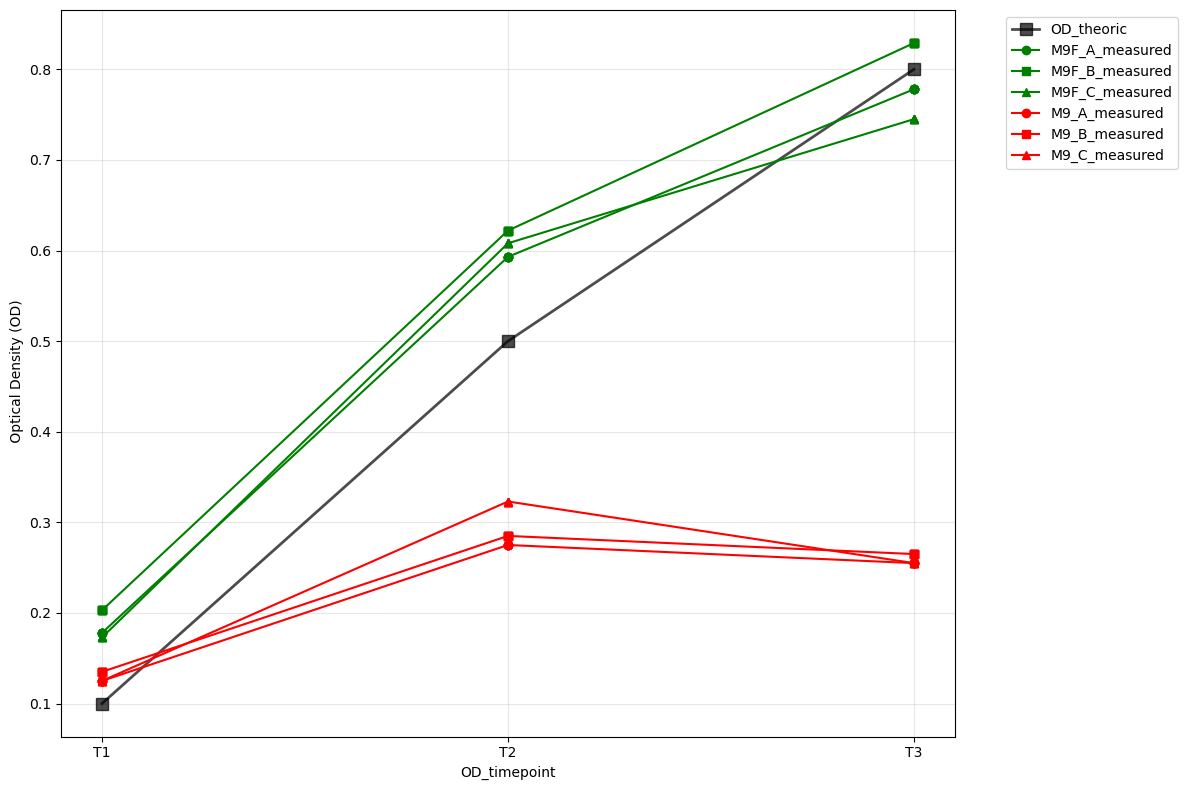
\includegraphics[keepaspectratio]{chapters/02-Materials-and-methods_files/figure-latex/..-data-data_growth-fig-growth-curves-output-1.png}}

}

\caption{\label{fig-growth-curves}Growth of the different bacterial
populations over time}

\end{figure}%

Growth curves for each condition showing the optical density (OD)
measurements over time for M9 and M9F media across three biological
replicates (Rep A, B, C) at three time points (T1, T2, T3).

The growth curves reveal distinct patterns between the two culture
conditions. Bacteria grown in M9F medium (high glucose and iron)
exhibited significantly higher growth rates and reached higher optical
densities (OD 0.17-0.21 at T1, 0.59-0.63 at T2, 0.74-0.83 at T3)
compared to M9 medium (low glucose and iron) which showed limited growth
(OD 0.13 at T1, 0.28-0.33 at T2, 0.26 at T3). While M9F cultures showed
continued growth from T2 to T3, the growth rate slowed down during this
period, indicating the beginning of transition towards stationary phase.
The M9 cultures appeared to reach a growth plateau by T3, while M9F
cultures maintained higher densities despite the growth deceleration,
suggesting nutrient limitation in the M9 condition. Biological
replicates showed excellent reproducibility validating the experimental
design.

Cells were collected at each timepoint (T1, T2, T3) from all biological
replicates for subsequent single-cell RNA-seq analysis using the
microSPLiT protocol.

\section{microSPLiT protocol}\label{microsplit-protocol}

\begin{figure}

\centering{

\pandocbounded{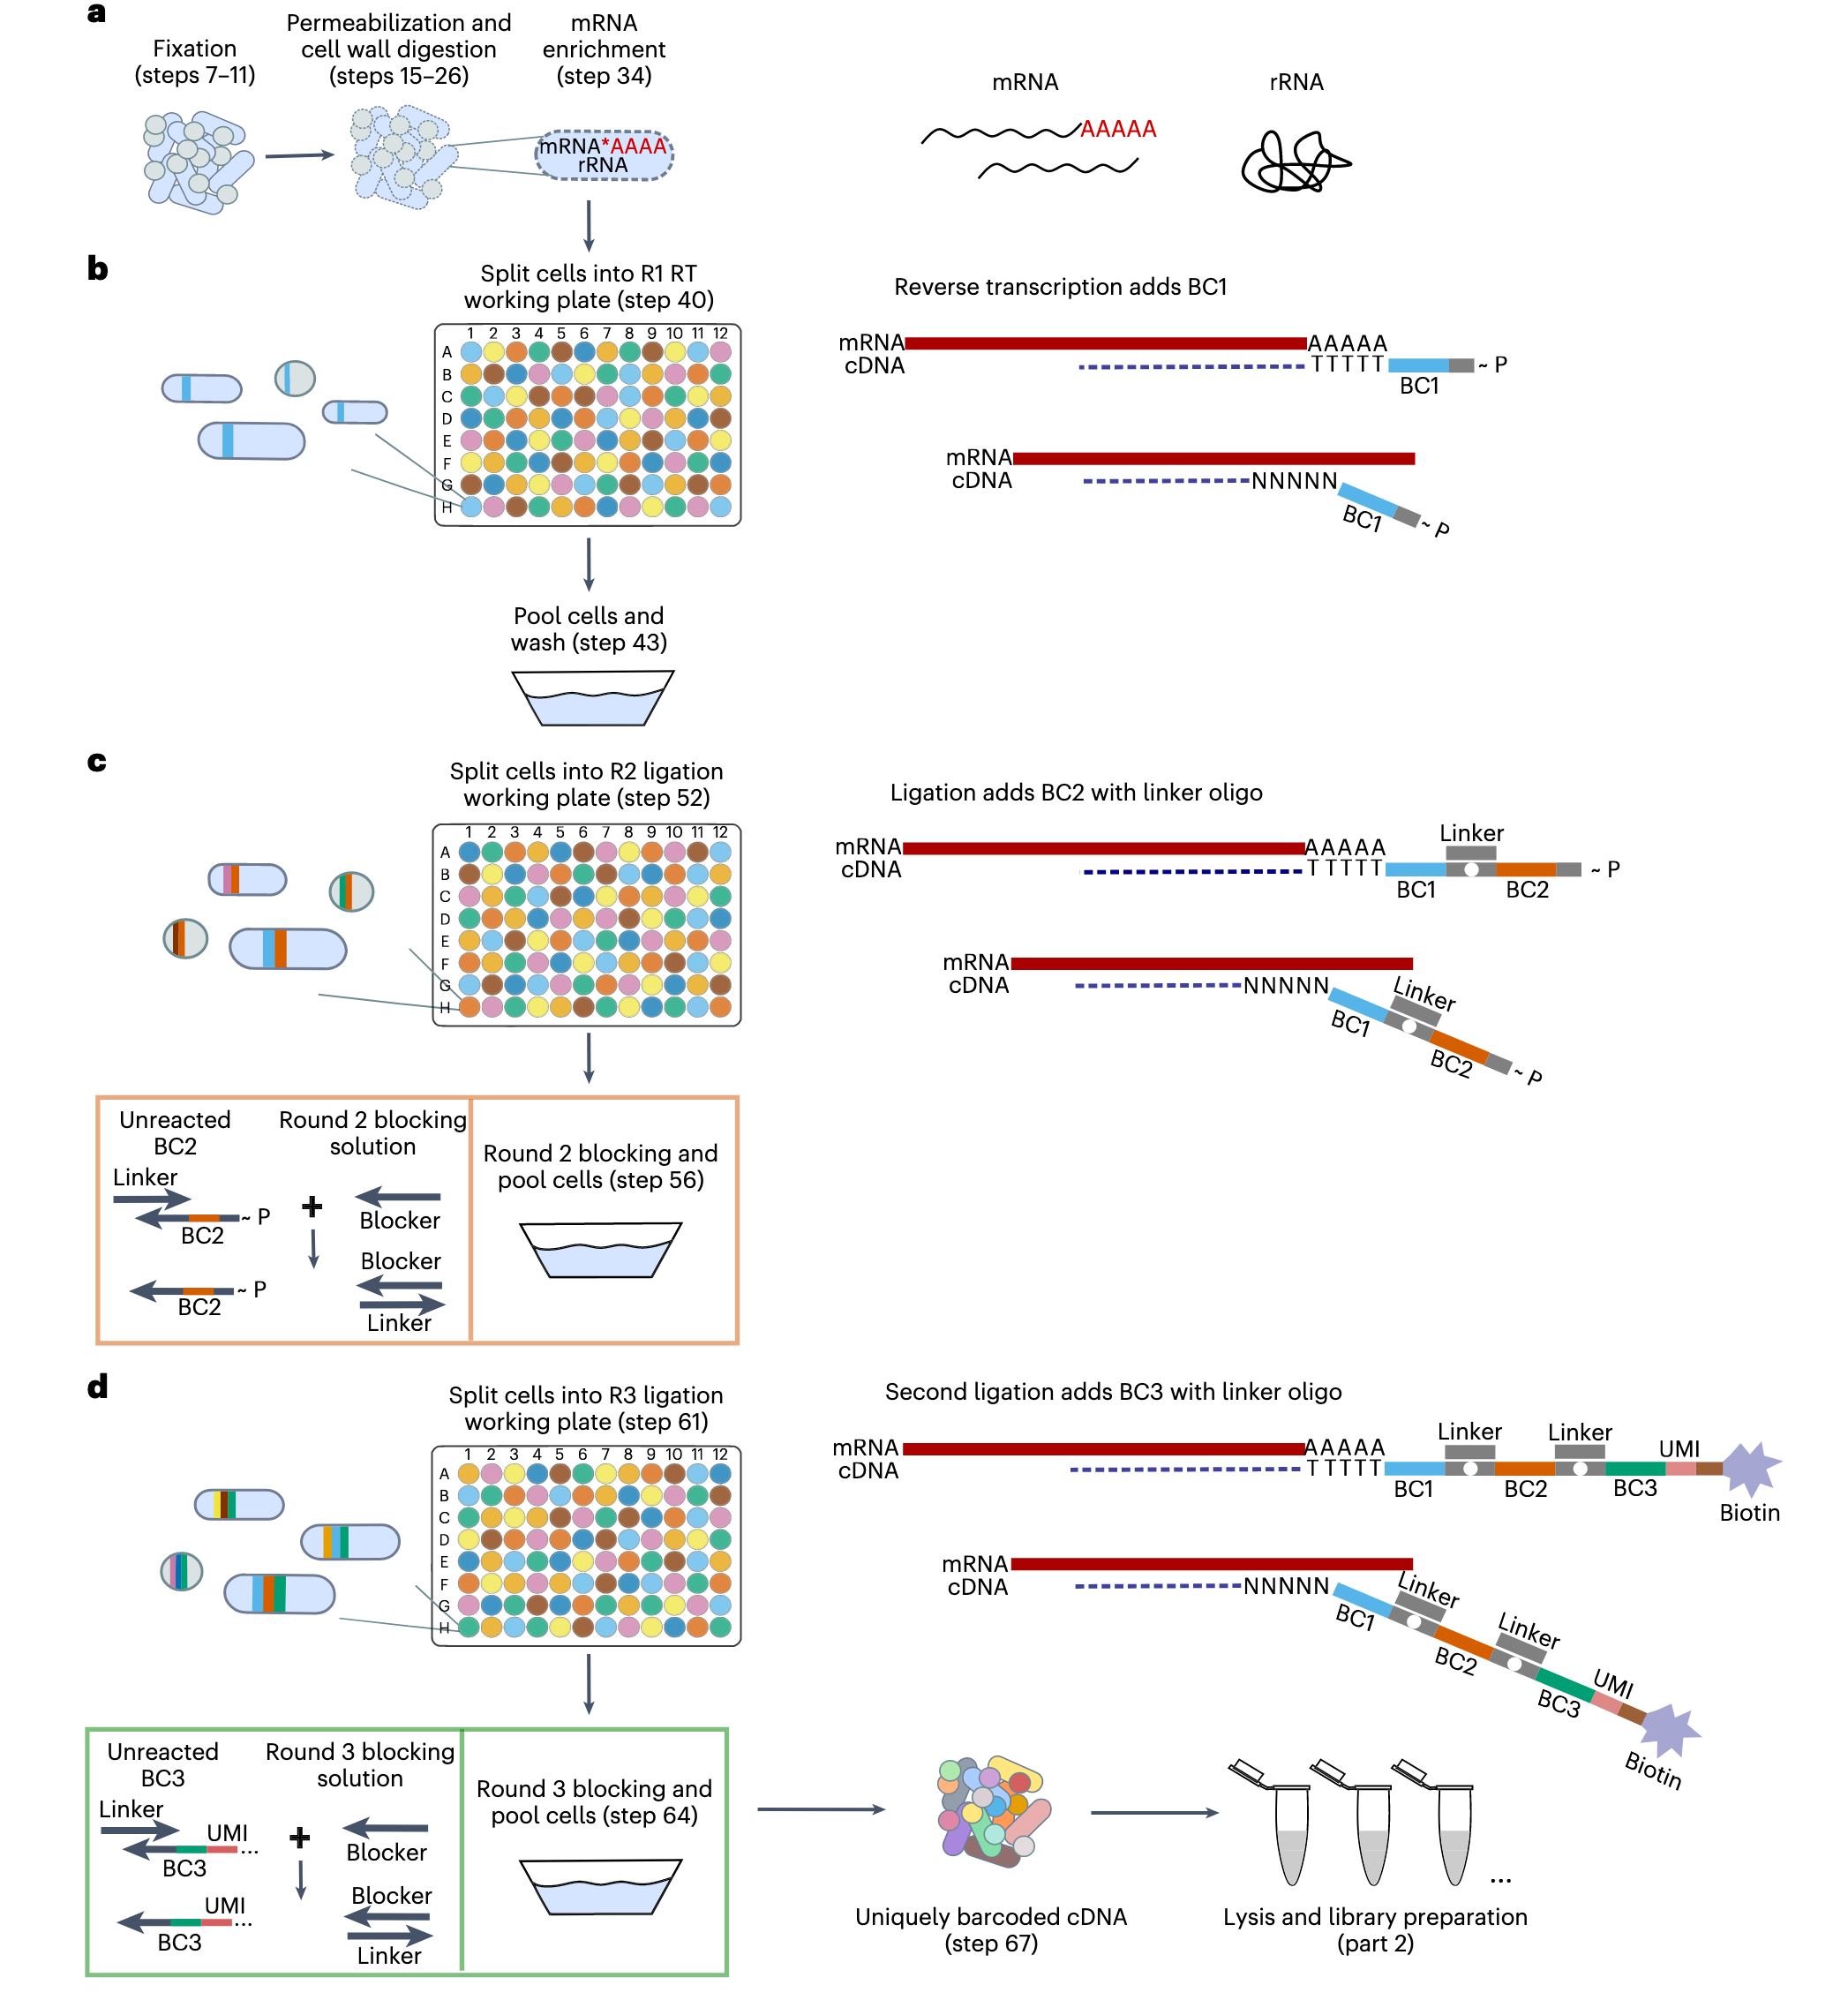
\includegraphics[keepaspectratio]{chapters/../figures/protocol.png}}

}

\caption{\label{fig-protocol}Schematic representation of the microSPLiT
protocol showing the barcoding workflow for single-cell
RNA-seq.\textsuperscript{\citeproc{ref-gaisser2024}{2}}}

\end{figure}%

pas fou rexpliquer en mieux et simple , juste focus sur elements
importants The microSPLiT (microbial Split-Pool Ligation
Transcriptomics) protocol enables single-cell RNA sequencing of bacteria
by performing barcoding reactions inside individual cells rather than in
separate reaction vessels . This approach maintains single-cell
resolution throughout the entire process, from cell fixation to library
preparation. The protocol involves multiple rounds of split-pool
barcoding where cells are distributed into 96-well plates, barcoded,
pooled, and redistributed for subsequent rounds, creating unique barcode
combinations that identify individual cells. This method allows for the
analysis of transcriptomic heterogeneity within bacterial populations at
single-cell resolution, providing insights into gene expression patterns
and cellular diversity that would be masked in bulk RNA-seq approaches.

\subsection{microSPLiT library and read
structure}\label{microsplit-library-and-read-structure}

split en 4 sous librairies pour meilleur sequençage

\section{Pipeline for microSPLiT data
processing}\label{pipeline-for-microsplit-data-processing}

\begin{figure}

\centering{

\includegraphics[width=6in,height=4in]{chapters/02-Materials-and-methods_files/figure-latex/mermaid-figure-2.png}

}

\caption{\label{fig-pipeline}Pipeline for microSPLiT data processing}

\end{figure}%

\subsection{Sequencing and demultiplexing of
libraries}\label{sequencing-and-demultiplexing-of-libraries}

Sequencing was performed on a NovaSeq instrument (Genobird platform)
using four different indexes, in paired-end mode. The sequencing
facility provided two types of files: raw Illumina BCL files (250 GB)
and demultiplexed paired-end FASTQ files (150 GB). For all downstream
analyses, only the demultiplexed FASTQ files were used, as the index
sequences had already been removed by the platform.

For each index, two paired-end FASTQ files were generated: - \textbf{R1}
contains the cDNA sequence of interest (transcriptome). - \textbf{R2}
contains the cell barcodes and unique molecular identifiers (UMIs).

\subsection{Quality control and
trimming}\label{quality-control-and-trimming}

All quality control, trimming, and alignment steps were performed on the
GenOuest high-performance computing cluster using SLURM job scripts to
ensure efficient and reproducible analysis of large-scale sequencing
data. \footnote{All analyses were performed on the GenOuest
  high-performance computing cluster (Rennes, France) using SLURM job
  scripts for automation and reproducibility.}

Read quality was initially assessed for all four libraries (R1 and R2)
using FastQC and MultiQC. Trimming was performed with
Cutadapt\textsuperscript{\citeproc{ref-martin2011}{8}} and
Fastp\textsuperscript{\citeproc{ref-chen2018}{9}} to retain only the
cDNA portion in R1 and to filter R2 for valid barcodes. After trimming,
read quality was reassessed with FastQC and MultiQC, and results were
merged for global quality evaluation.

Read trimming followed a custom multi-step pipeline (see Appendix Table
Table~\ref{tbl-tso-removal} and Section
Section~\ref{sec-appendix-trimming-steps} for details):

\begin{itemize}
\tightlist
\item
  \textbf{TSO trimming (R1 only):} Removal of template-switching oligo
  (TSO) sequences from the 5' end of cDNA reads using Cutadapt (24--28\%
  of reads affected).
\item
  \textbf{Initial quality and polyG/polyX trimming (R1 and R2):} Removal
  of low-quality bases and polyG/polyX tails with Fastp, addressing
  artifacts from two-color chemistry.
\item
  \textbf{PolyA trimming (R1 only):} Removal of polyA stretches (≥15 nt)
  from R1 using Cutadapt, targeting protocol-specific artifacts.
\item
  \textbf{Adapter and linker trimming (R1 only):} Sequential removal of
  specific adapters and linker sequences (e.g., CCACAGTCTCAAGCAC,
  AGTCGTACGCCGATGCGAAACATCGGCCAC, AGATCGGAAGAGCACACGTCTGAACTCCAGTCA)
  with Cutadapt, including those from random hexamer priming.
\item
  \textbf{Final quality and length filtering (R1 and R2):} Additional
  filtering with Fastp to retain only high-quality, sufficiently long
  reads.
\end{itemize}

All steps were performed in paired-end mode to maintain synchronization
between R1 and R2. The pipeline is fully automated, SLURM-compatible,
and resource usage was monitored for each sample. For the complete
pipeline and command details, see Appendix Section
Section~\ref{sec-appendix-trimming-steps}.

\subsection{STARsolo alignment and barcode
reading}\label{starsolo-alignment-and-barcode-reading}

\begin{verbatim}
-   demultiplexage des index de librairies (réalisé par la plateforme de sequençage)

-   QC control des données avec Andrews, S. (2010). FastQC:  A Quality Control Tool for High Throughput Sequence Data [Online]. Available online at: <http://www.bioinformatics.babraham.ac.uk/projects/fastqc/> et avec [@ewels2016]

-   trimming des données de seqeunçage avec Fastp [@chen2018] et Cutadapt [@martin2011]

-   aligment des data sur le genome de reference de *Pseudomonas brassicacearum* grace à STARsolo un amelioration de l'outils STAR pour les données single-cell [@dobin2013][@kaminow]

-   different other tools existe comme pour alignement et lecture des barcodes SPLiTseq/ microSPliT comme Kallisto [@bray2016], [@sullivan2025] mais d'apres le benchmarking de le plus rapide, reproductible est starsolo [@kuijpers2024]
\end{verbatim}

\bookmarksetup{startatroot}

\chapter{Results}\label{results}

\begin{itemize}
\tightlist
\item
  4 libraries of unequal sizes (see Solène's explanation for why they
  were not exactly equivalent)
\item
  This impacts library efficiency
\item
  =\textgreater{} Recommendation: balance the libraries for optimal
  results
\end{itemize}

\section{Stats sur les reads R1 et R2
:}\label{stats-sur-les-reads-r1-et-r2}

\begin{itemize}
\tightlist
\item
  On a subset of 1,000,000 reads:

  \begin{itemize}
  \tightlist
  \item
    Percentage of reads containing TSO
  \item
    Percentage of reads containing polyA
  \item
    Percentage of reads containing adapter
  \item
    Percentage of reads containing linker -\textgreater{} possibly in
    appendix
  \end{itemize}
\end{itemize}

Reminder about saturation calculation method:

\section{Trimming}\label{trimming}

ici j'ai suivi les recommendations de kuchina , seulement presenté les
resultats Genfull , mettre plus tard les resultats de Gene

\begin{itemize}
\tightlist
\item
  renvoie vers l'annexe pour les multiqc (fastp, cutadapt) avant et
  apres trimming
\item
\item
  mais au final on obtient des resultats tres interessants et propres
\end{itemize}

=\textgreater{} peut etre il aurait été interressant de faire un
trimming comme kuchina 2021 pour comparer les resultats =\textgreater{}
renvoie vers la discussion pour le trimming fait dans l'article
de\textsuperscript{\citeproc{ref-kuchina2021}{1}} - avait presque 90\%
de saturation =\textgreater{} a verifier si c'est vraiment le cas - et
10 \% des sequences avec TSO (voir Annexe)

\begin{itemize}
\tightlist
\item
  Summary table of Starsolo results
\item
  numbers of reads before and after trimming
\item
  taux de saturation \ldots{}
\item
  =\textgreater{} renvoie vers la discussion pour les taux de saturation
\end{itemize}

\section{STARsolo}\label{starsolo}

-pour starsolo renvoie un gene qui serait mal annoté donc est
automatiquement ignoré

commande starsolo suivante comme dans bretn permet UMI a une
erreur\ldots{} possition des barcodes

\section{Genome}\label{genome}

\section{Transcriptome}\label{transcriptome}

\bookmarksetup{startatroot}

\chapter{Fitrage des cellules}\label{fitrage-des-cellules}

\begin{itemize}
\item
  reflexion sur le filtrages des cellules est complexe : comme
  mentionnée dans l'article de il existe des methodes de filtrages plus
  ou moins complexes\\
  -filtrage sur le types de reads, globales ou seuils differents entre
  les differentes conditions biologiques -filtrage sur le nombre de
  reads par cellule -filtrage sur le nombre de genes exprimés par
  cellule -filtrage sur le nombre de reads par gene
\item
  filtrage avec un threashold
\item
  dans l'article de kuchina 2021 , ils ont utilisé un seuil de 200 UMI
  par cellule
\item
\item
  preprint de \ldots{} pourrait etre interessant de se focus aussi sur
  rRNA (lien avec growth rate)
\end{itemize}

\bookmarksetup{startatroot}

\chapter{}\label{section}

housekeeping genes

choix ou non de pooler les replicas techniques ensembles

\section{Summary of results}\label{summary-of-results}

\section{MultiQC Quality Reports}\label{multiqc-quality-reports}

Detailed sequence quality reports are available below. Click on each
report to view it.

\subsubsection{MultiQC Report R1 Before Trimming}

Click to view MultiQC report R1 before trimming

\subsubsection{MultiQC Report R1 After Trimming}

Click to view MultiQC report R1 after trimming

\subsubsection{MultiQC Report R2 Before Trimming}

Click to view MultiQC report R2 before trimming

\subsubsection{MultiQC Report R2 After Trimming}

Click to view MultiQC report R2 after trimming

Key quality metrics are summarized in the tables below.

\begin{table}

\caption{\label{tbl-example}Before trimming}

\begin{minipage}{\linewidth}

\begin{longtable}[]{@{}lllll@{}}
\toprule\noalign{}
Sample Name & Dups & GC & Median len & Seqs \\
\midrule\noalign{}
\endhead
\bottomrule\noalign{}
\endlastfoot
BC\_0076\_R1 & 94.5\% & 55.0\% & 241bp & 631.4M \\
BC\_0077\_R1 & 94.1\% & 53.0\% & 241bp & 325.5M \\
BC\_0079\_R1 & 93.8\% & 53.0\% & 241bp & 379.1M \\
BC\_0080\_R1 & 94.6\% & 54.0\% & 241bp & 397.7M \\
\textbf{Total} & - & - & - & \textbf{1,733.7M} \\
\end{longtable}

\end{minipage}%

\end{table}%

\begin{table}

\caption{\label{tbl-example}After trimming}

\begin{minipage}{\linewidth}

\begin{longtable}[]{@{}lllll@{}}
\toprule\noalign{}
Sample Name & Dups & GC & Median len & Seqs \\
\midrule\noalign{}
\endhead
\bottomrule\noalign{}
\endlastfoot
BC\_0076\_R1 & 98.7\% & 51.0\% & 127bp & 450.8M \\
BC\_0077\_R1 & 98.6\% & 51.0\% & 157bp & 248.4M \\
BC\_0079\_R1 & 98.6\% & 51.0\% & 152bp & 285.2M \\
BC\_0080\_R1 & 98.7\% & 51.0\% & 132bp & 300.1M \\
\textbf{Total} & - & - & - & \textbf{1,284.5M} \\
\end{longtable}

\end{minipage}%

\end{table}%

\begin{table}

\caption{\label{tbl-summary}Summary of sequence metrics before and after
trimming, including percentage changes}

\begin{minipage}{\linewidth}

\begin{longtable}[]{@{}
  >{\raggedright\arraybackslash}p{(\linewidth - 12\tabcolsep) * \real{0.1429}}
  >{\raggedright\arraybackslash}p{(\linewidth - 12\tabcolsep) * \real{0.1429}}
  >{\raggedright\arraybackslash}p{(\linewidth - 12\tabcolsep) * \real{0.1429}}
  >{\raggedright\arraybackslash}p{(\linewidth - 12\tabcolsep) * \real{0.1429}}
  >{\raggedright\arraybackslash}p{(\linewidth - 12\tabcolsep) * \real{0.1429}}
  >{\raggedright\arraybackslash}p{(\linewidth - 12\tabcolsep) * \real{0.1429}}
  >{\raggedright\arraybackslash}p{(\linewidth - 12\tabcolsep) * \real{0.1429}}@{}}
\toprule\noalign{}
\begin{minipage}[b]{\linewidth}\raggedright
Sample Name
\end{minipage} & \begin{minipage}[b]{\linewidth}\raggedright
Before Trimming
\end{minipage} & \begin{minipage}[b]{\linewidth}\raggedright
\end{minipage} & \begin{minipage}[b]{\linewidth}\raggedright
After Trimming
\end{minipage} & \begin{minipage}[b]{\linewidth}\raggedright
\end{minipage} & \begin{minipage}[b]{\linewidth}\raggedright
Change in
\end{minipage} & \begin{minipage}[b]{\linewidth}\raggedright
\end{minipage} \\
\midrule\noalign{}
\endhead
\bottomrule\noalign{}
\endlastfoot
& Median len & Seqs & Median len & Seqs & Length & Sequences \\
-------------- & ---------------- & ------------ & ---------------- &
------------ & ----------- & ----------- \\
BC\_0076\_R1 & 241bp & 631.4M & 127bp & 450.8M & -47.3\% & -28.6\% \\
BC\_0077\_R1 & 241bp & 325.5M & 157bp & 248.4M & -34.9\% & -23.7\% \\
BC\_0079\_R1 & 241bp & 379.1M & 152bp & 285.2M & -36.9\% & -24.8\% \\
BC\_0080\_R1 & 241bp & 397.7M & 132bp & 300.1M & -45.2\% & -24.5\% \\
\textbf{Mean} & \textbf{241bp} & \textbf{433.4M} & \textbf{142bp} &
\textbf{321.1M} & - & - \\
\textbf{Total} & - & \textbf{1733.7M} & - & \textbf{1284.5M} &
\textbf{-41.1\%} & \textbf{-25.4\%} \\
\end{longtable}

\end{minipage}%

\end{table}%

\begin{table}

\caption{\label{tbl-starsolo}STARsolo barcode statistics}

\begin{minipage}{\linewidth}

\begin{longtable}[]{@{}ll@{}}
\toprule\noalign{}
Metric & Count \\
\midrule\noalign{}
\endhead
\bottomrule\noalign{}
\endlastfoot
nNoAdapter & 0 \\
nNoUMI & 0 \\
nNoCB & 67,177 \\
nNinCB & 0 \\
nNinUMI & 16,893,550 \\
nUMIhomopolymer & 1,697,129 \\
nTooMany & 0 \\
nNoMatch & 163,166,830 \\
nMismatchesInMultCB & 3,323,192 \\
nExactMatch & 1,046,121,284 \\
nMismatchOneWL & 53,206,471 \\
nMismatchToMultWL & 0 \\
\end{longtable}

\end{minipage}%

\end{table}%

\subsection{Barcode Statistics
Interpretation}\label{barcode-statistics-interpretation}

The analysis of cell barcodes reveals several important points about our
data quality:

\begin{itemize}
\tightlist
\item
  \textbf{Barcode Quality}:

  \begin{itemize}
  \tightlist
  \item
    The absence of reads without adapter (\texttt{nNoAdapter\ =\ 0}) and
    without UMI (\texttt{nNoUMI\ =\ 0}) indicates excellent library
    preparation quality
  \item
    The relatively low number of reads without cell barcode
    (\texttt{nNoCB\ =\ 67,177}) represents less than 0.01\% of total
    reads, which is excellent
  \end{itemize}
\item
  \textbf{Barcode Accuracy}:

  \begin{itemize}
  \tightlist
  \item
    The majority of reads (1,046,121,284) have a perfectly aligned
    barcode (\texttt{nExactMatch})
  \item
    Approximately 53 million reads show a single mismatch
    (\texttt{nMismatchOneWL})
  \item
    The absence of reads with multiple matches
    (\texttt{nMismatchToMultWL\ =\ 0}) suggests good barcode specificity
  \end{itemize}
\item
  \textbf{UMI Quality}:

  \begin{itemize}
  \tightlist
  \item
    The number of invalid UMIs (\texttt{nNinUMI\ =\ 16,893,550})
    represents a relatively small proportion of total reads and might be
    primarily due to sequencing errors at the beginning of reads, which
    is a common observation in Illumina sequencing
  \item
    The presence of homopolymers in UMIs
    (\texttt{nUMIhomopolymer\ =\ 1,697,129}) is a known phenomenon that
    can affect molecular counting accuracy, but the relatively low
    number suggests this is not a major concern
  \end{itemize}
\item
  \textbf{Overall Matching}:

  \begin{itemize}
  \tightlist
  \item
    The significant number of unmatched reads
    (\texttt{nNoMatch\ =\ 163,166,830}) suggests that a substantial
    portion of reads do not match expected barcodes
  \item
    This could be due to sequencing errors or potential contamination
  \end{itemize}
\end{itemize}

These results indicate overall good library preparation quality, with
excellent cell barcode specificity, although some improvements could be
made regarding UMI quality.

\section{Genfull}\label{genfull}

\begin{table}

\caption{\label{tbl-starsolo-features}STARsolo feature mapping
statistics}

\begin{minipage}{\linewidth}

\begin{longtable}[]{@{}ll@{}}
\toprule\noalign{}
Metric & Count \\
\midrule\noalign{}
\endhead
\bottomrule\noalign{}
\endlastfoot
nUnmapped & 114,628,761 \\
nNoFeature & 13,153,735 \\
nAmbigFeature & 936,951,032 \\
nAmbigFeatureMultimap & 935,077,136 \\
nTooMany & 0 \\
nNoExactMatch & 125,216 \\
nExactMatch & 4,471,174,098 \\
nMatch & 971,519,404 \\
nMatchUnique & 34,593,349 \\
nCellBarcodes & 699,355 \\
nUMIs & 34,258,961 \\
\end{longtable}

\end{minipage}%

\end{table}%

\subsection{Detailed Interpretation of STARsolo
Statistics}\label{detailed-interpretation-of-starsolo-statistics}

Based on the official STAR documentation and explanations from Alex
Dobin (STAR developer)
\href{https://github.com/alexdobin/STAR/issues/1887}{\textsuperscript{\citeproc{ref-alexdobinux2fSTARux5cux231887}{\textbf{alexdobin/STAR\#1887?}}}},
here is a detailed interpretation of our STARsolo statistics:

\subsubsection{Barcode Statistics
(Barcodes.stats)}\label{barcode-statistics-barcodes.stats}

Statistics with the ``no'' prefix indicate reads that are not used for
quantification:

\begin{itemize}
\tightlist
\item
  \textbf{Barcode Quality} :

  \begin{itemize}
  \tightlist
  \item
    \texttt{nNoAdapter} : Reads without adapter
  \item
    \texttt{nNoUMI} : Reads without valid UMI
  \item
    \texttt{nNoCB} : Reads without valid cell barcode
  \item
    \texttt{nNinCB} : Reads with `N' bases in cell barcode
  \item
    \texttt{nNinUMI} : Reads with `N' bases in UMI
  \item
    \texttt{nUMIhomopolymer} : Reads with homopolymeric UMI
  \end{itemize}
\end{itemize}

\subsubsection{Mapping Statistics
(Features.stats)}\label{mapping-statistics-features.stats}

These statistics refer to the number of reads, except for
\texttt{nCellBarcodes} and \texttt{nUMIs} which represent the number of
valid cell barcodes and UMIs respectively.

\begin{itemize}
\tightlist
\item
  \textbf{General Mapping} :

  \begin{itemize}
  \tightlist
  \item
    \texttt{nUnmapped} : Reads not mapped to the genome
  \item
    \texttt{nNoFeature} : Reads not mapped to an annotated feature
  \item
    \texttt{nAmbigFeature} : Reads mapped to multiple features
  \item
    \texttt{nAmbigFeatureMultimap} : Subset of \texttt{nAmbigFeature}
    where reads are mapped to multiple genomic loci
  \end{itemize}
\item
  \textbf{Mapping Quality} :

  \begin{itemize}
  \tightlist
  \item
    \texttt{nExactMatch} : Reads with exact mapping
  \item
    \texttt{nMatch} : Total mapped reads (unique + multiple)
  \item
    \texttt{nMatchUnique} : Reads with unique mapping
  \end{itemize}
\end{itemize}

\subsubsection{Sequencing Saturation}\label{sequencing-saturation}

Sequencing saturation is calculated as follows:

\begin{verbatim}
Saturation = 1 - (N_umi / N_reads)
\end{verbatim}

where: - N\_umi = number of unique CB/UMI/gene combinations - N\_reads =
number of reads with valid CB/UMI/gene

In our case, the very low saturation (0.97\%) indicates that we could
sequence deeper to capture more unique molecules.

\subsubsection{Key Points of Our
Analysis}\label{key-points-of-our-analysis}

\begin{itemize}
\tightlist
\item
  The high number of ambiguous mappings
  (\texttt{nAmbigFeature\ =\ 936,951,032}) is typical for bacterial data
  due to the compact nature of the genome
\item
  The majority of reads have exact mapping
  (\texttt{nExactMatch\ =\ 4,471,174,098}), indicating good mapping
  quality. This possibly includes both unique and multi-mapped reads
  that match exactly to their reference locations
\item
  The number of detected cell barcodes
  (\texttt{nCellBarcodes\ =\ 699,355}) is high, suggesting good cellular
  diversity
\item
  The number of UMIs (\texttt{nUMIs\ =\ 34,258,961}) indicates good
  molecular coverage
\end{itemize}

These metrics suggest that our data is of good technical quality,
although the low saturation indicates potential for deeper sequencing.

\section{Genefull summary stats}\label{genefull-summary-stats}

\begin{table}

\caption{\label{tbl-starsolo-summary}STARsolo summary statistics}

\begin{minipage}{\linewidth}

\begin{longtable}[]{@{}ll@{}}
\toprule\noalign{}
Metric & Value \\
\midrule\noalign{}
\endhead
\bottomrule\noalign{}
\endlastfoot
Number of Reads & 1,284,475,633 \\
Reads With Valid Barcodes & 85.58\% \\
Sequencing Saturation & 0.97\% \\
Q30 Bases in CB+UMI & 95.51\% \\
Q30 Bases in RNA read & 95.79\% \\
Reads Mapped to Genome: Unique+Multiple & 89.57\% \\
Reads Mapped to Genome: Unique & 3.64\% \\
Reads Mapped to GeneFull: Unique+Multiple & 75.64\% \\
Reads Mapped to GeneFull: Unique & 2.69\% \\
Estimated Number of Cells & 27,203 \\
Unique Reads in Cells Mapped to GeneFull & 12,794,311 \\
Fraction of Unique Reads in Cells & 36.98\% \\
Mean Reads per Cell & 470 \\
Median Reads per Cell & 381 \\
UMIs in Cells & 12,663,144 \\
Mean UMI per Cell & 465 \\
Median UMI per Cell & 378 \\
Mean GeneFull per Cell & 296 \\
Median GeneFull per Cell & 258 \\
Total GeneFull Detected & 6,035 \\
\end{longtable}

\end{minipage}%

\end{table}%

\section{Interpretation of STARsolo
Results}\label{interpretation-of-starsolo-results}

The STARsolo analysis revealed several key insights about our
single-cell RNA-seq data:

\subsection{Sequencing Quality and
Mapping}\label{sequencing-quality-and-mapping}

\begin{itemize}
\tightlist
\item
  The sequencing quality is excellent, with over 95\% of bases having
  Q30 quality scores in both barcode/UMI and RNA reads
\item
  A high proportion (85.58\%) of reads contained valid cell barcodes,
  indicating good library preparation
\item
  The mapping rates are robust:

  \begin{itemize}
  \tightlist
  \item
    89.57\% of reads mapped to the genome (unique + multiple)
  \item
    75.64\% of reads mapped to genes (unique + multiple)
  \end{itemize}
\item
  The low unique mapping rate (3.64\% to genome, 2.69\% to genes) is
  typical for bacterial RNA-seq due to \ldots{}
\end{itemize}

\subsection{Mapping Terminology}\label{mapping-terminology}

\begin{itemize}
\tightlist
\item
  \textbf{Gene mapping}: Refers to reads mapped to annotated coding
  sequences (CDS) only
\item
  \textbf{GeneFull mapping}: Includes reads mapped to all annotated
  features including:

  \begin{itemize}
  \tightlist
  \item
    Coding sequences (CDS)
  \item
    Untranslated regions (UTRs)
  \item
    Non-coding RNAs
  \item
    Intergenic regions
  \item
    This broader mapping approach is particularly relevant for bacterial
    transcriptomics as it captures the full complexity of the
    transcriptome
  \end{itemize}
\end{itemize}

\subsection{Cell Recovery and
Expression}\label{cell-recovery-and-expression}

\begin{itemize}
\tightlist
\item
  We estimated 27,203 cells in our dataset
\item
  The sequencing saturation is very low (0.97\%), suggesting we could
  sequence deeper if needed
\item
  Cell-level metrics show good coverage:

  \begin{itemize}
  \tightlist
  \item
    Mean/median reads per cell: 470/381
  \item
    Mean/median UMIs per cell: 465/378
  \item
    Mean/median genes per cell: 296/258
  \end{itemize}
\item
  We detected 6,035 genes in total across all cells
\end{itemize}

\subsection{Data Quality Assessment}\label{data-quality-assessment}

\begin{itemize}
\tightlist
\item
  The high Q30 scores and mapping rates indicate good technical quality
\item
  The cell-level metrics suggest sufficient coverage for downstream
  analysis
\item
  The low sequencing saturation suggests potential for deeper sequencing
  if needed
\item
  The high proportion of reads with valid barcodes (85.58\%) indicates
  good library preparation
\end{itemize}

\subsection{filter}\label{filter}

Nous on prend tout les barcodes pas ceux qui sont filtré donc les 820,
800 barcodes

\section{apres starsolo mettre le nombre de reads avec valid barcodes
dans la
table}\label{apres-starsolo-mettre-le-nombre-de-reads-avec-valid-barcodes-dans-la-table}

\subsection{genome}\label{genome-1}

circular representation of c-bacterial genome and read alignment voir
comment faire ce type de figure et l'article qui l'avait fait

\subsection{}\label{section-1}

Attention j'ai filtré pour ne garder que les CDS mais certains pas
annotés plutot exclure les tRNA et rRNA

In addition, we kept the highest-scored multimapping reads, assigning a
fractional count based on the number of equally good alignments, because
bacterial genomes are known to contain overlapping coding sequences. We
then generated a matrix of gene counts for each cell (N-by-K matrix,
with N cells and K genes).

dans l'article de kuchina ils ont filtré les cellules en fonction du
nombre de reads et de genes :

``Processing of data from the heat shock experiment Clustering and data
analysis for the speciesmixing experiment with heat shock treatment was
performed using Scanpy (59). We only kept transcriptomes that had a
\textbf{number of total reads higher than 200}. Then, we removed the
\textbf{ribosomal and tRNA reads from the data}, retaining only reads
that represented the mRNA counts for both species. We further filtered
cells based on the mRNA counts, \textbf{retaining cells expressing
\textgreater100 reads and \textgreater100 genes}, and additionally
filtered the genes, retaining the \textbf{genes expressed in
\textgreater5 cells}. We then applied standard Scanpy normalization and
scaling, dimensionality reduction, and clustering, as described in the
Scanpy tutorial (59, 60). The clusters were produced by the Louvain
graph-clustering method and manually inspected for the top
differentially expressed genes. After inspection, three pairs of
transcriptionally similar clusters with fewer differentially expressed
genes were merged, resulting in clusters 1, 2, and 3 in Fig. 1D.''
(\href{zotero://select/library/items/AWDKBVJW}{Kuchina et al., 2021,
p.~8})
(\href{zotero://open-pdf/library/items/YFM8QJY6?page=9&annotation=LXF2XHIY}{pdf})

\bookmarksetup{startatroot}

\chapter{Initialize the Seurat object with the raw (non-normalized
data).}\label{initialize-the-seurat-object-with-the-raw-non-normalized-data.}

pbmc \textless- CreateSeuratObject(counts = pbmc.data, project =
``pbmc3k'', min.cells = 3, min.features = 200)

https://rnabioco.github.io/cellar/previous/2019/docs/2\_filtering\_QC.html

\section{Overview}\label{overview}

This chapter presents the findings of our single-cell RNA-seq analysis
of Pseudomonas, focusing on the division of labor within bacterial
populations.

\section{Single-cell RNA-seq
Analysis}\label{single-cell-rna-seq-analysis}

\subsection{Data Quality and
Preprocessing}\label{data-quality-and-preprocessing}

\subsection{Cell Type Identification}\label{cell-type-identification}

\subsection{Differential Expression
Analysis}\label{differential-expression-analysis}

\subsection{Division of Labor
Patterns}\label{division-of-labor-patterns}

\section{Functional Analysis}\label{functional-analysis}

\subsection{Pathway Enrichment}\label{pathway-enrichment}

\subsection{Gene Set Analysis}\label{gene-set-analysis}

\subsection{Regulatory Network
Analysis}\label{regulatory-network-analysis}

\section{Integration with Previous
Studies}\label{integration-with-previous-studies}

\section{Summary of Key Findings}\label{summary-of-key-findings}

\bookmarksetup{startatroot}

\chapter{Discussion}\label{discussion}

We applied microSPLiT to P. brassicacearum growing in two different
conditions in rich medium (M9F) and in minimal medium (M9).

\begin{itemize}
\item
  recepetion tardives des resultats
\item
  mis beaucoup de temps pour le trimming ( 1mois) le temps de comprendre
  la structure de la librairie et
\item
\item
\item
  analyse temporelle , metabolique , bulkRNAseq
\item
  utilisation pour capturer specifique mRNA (voir article : 2 methodes
  existes ; et apres aussi peut etre fait )
\item
  mais je pense deja bioinformatiquement on peut faire des choses pour
  ameliorer reads utilisables
\item
  comparer avec differentes methodes de single cell RNA seq, voir si on
  observe toujours la meme chose ou pas
\item
  versionnement des outils utilisés (renv , singularity, conda)
\item
  rapport fait un template pour rendu propre
\item
\end{itemize}

autres outils pourrait etre ajouter dans le pipeline comme BarQC
alternative à Starsolo pour meilleur la lecture des barcodes (en
considerant utilisant des positions non fixe (CIGAR motif) et evaluer la
qualité UMIs et
repartitions\textsuperscript{\citeproc{ref-rossello}{10}},

pour la qualité et contamination : centriguge et
recentrifuge\textsuperscript{\citeproc{ref-martuxed2019}{11},\citeproc{ref-kim2016}{12}}

meme si moins de risque de contamination car cellules fixé \ldots{}
(deve

\begin{itemize}
\tightlist
\item
  Nextflow pour le trimming, QC , et STARsolo serait une bonne idée , et
  barQC ; pourrait etre utile pour la communauté
\end{itemize}

-autono -gestion des datas tailles des \#\# Interpretation of Key
Findings

\subsection{Division of Labor
Mechanisms}\label{division-of-labor-mechanisms}

\subsection{Biological Significance}\label{biological-significance}

\subsection{Technical Considerations}\label{technical-considerations}

\section{Comparison with Existing
Literature}\label{comparison-with-existing-literature}

\subsection{Similarities with Previous
Studies}\label{similarities-with-previous-studies}

\subsection{Novel Insights}\label{novel-insights}

\subsection{Discrepancies and Their
Implications}\label{discrepancies-and-their-implications}

\section{Methodological Strengths and
Limitations}\label{methodological-strengths-and-limitations}

\subsection{Technical Advantages}\label{technical-advantages}

\subsection{Potential Limitations}\label{potential-limitations}

\subsection{Future Methodological
Improvements}\label{future-methodological-improvements}

\section{Biological Implications}\label{biological-implications}

\subsection{Ecological Significance}\label{ecological-significance}

\subsection{Evolutionary Perspectives}\label{evolutionary-perspectives}

\subsection{Potential Applications}\label{potential-applications}

\section{Future Research Directions}\label{future-research-directions}

\subsection{Open Questions}\label{open-questions}

\subsection{Suggested Follow-up
Studies}\label{suggested-follow-up-studies}

\subsection{Technical Improvements}\label{technical-improvements}

\section{Conclusion}\label{conclusion}

\bookmarksetup{startatroot}

\chapter{Conclusion and Future Work}\label{conclusion-and-future-work}

\section{Summary of Main Findings}\label{summary-of-main-findings}

\subsection{Key Discoveries}\label{key-discoveries}

\subsection{Methodological
Contributions}\label{methodological-contributions}

\subsection{Biological Insights}\label{biological-insights}

\section{Impact on the Field}\label{impact-on-the-field}

\subsection{Contribution to Single-cell RNA-seq
Methodology}\label{contribution-to-single-cell-rna-seq-methodology}

\subsection{Contribution to Pseudomonas
Research}\label{contribution-to-pseudomonas-research}

\subsection{Broader Implications for Microbial
Ecology}\label{broader-implications-for-microbial-ecology}

\section{Future Research Directions}\label{future-research-directions-1}

\subsection{Technical Improvements}\label{technical-improvements-1}

\subsection{Biological Questions to
Address}\label{biological-questions-to-address}

\subsection{Potential Applications}\label{potential-applications-1}

\section{Final Remarks}\label{final-remarks}

\section{References}\label{references}

\clearpage
% Désactiver l'inclusion des prochaines figures et tableaux dans les listes
\captionsetup[figure]{list=false}
\captionsetup[table]{list=false}

\bookmarksetup{startatroot}

\chapter*{Bibliography}\label{bibliography}
\addcontentsline{toc}{chapter}{Bibliography}

\markboth{Bibliography}{Bibliography}

\phantomsection\label{refs}
\begin{CSLReferences}{0}{0}
\bibitem[\citeproctext]{ref-kuchina2021}
\CSLLeftMargin{1. }%
\CSLRightInline{Kuchina, A. \emph{et al.}
\href{https://doi.org/10.1126/science.aba5257}{Microbial single-cell RNA
sequencing by split-pool barcoding}. \emph{Science} \textbf{371},
eaba5257 (2021).}

\bibitem[\citeproctext]{ref-gaisser2024}
\CSLLeftMargin{2. }%
\CSLRightInline{Gaisser, K. D. \emph{et al.}
\href{https://doi.org/10.1038/s41596-024-01007-w}{High-throughput
single-cell transcriptomics of bacteria using combinatorial barcoding}.
\emph{Nature Protocols} \textbf{19}, 3048--3084 (2024).}

\bibitem[\citeproctext]{ref-morris2012}
\CSLLeftMargin{3. }%
\CSLRightInline{Morris, J. J., Lenski, R. E. \& Zinser, E. R.
\href{https://doi.org/10.1128/mBio.00036-12}{The black queen hypothesis:
Evolution of dependencies through adaptive gene loss}. \emph{mBio}
\textbf{3}, e00036--12 (2012).}

\bibitem[\citeproctext]{ref-morris2014}
\CSLLeftMargin{4. }%
\CSLRightInline{Morris, E. K. \emph{et al.}
\href{https://doi.org/10.1002/ece3.1155}{Choosing and using diversity
indices: insights for ecological applications from the German
Biodiversity Exploratories}. \emph{Ecology and Evolution} \textbf{4},
3514--3524 (2014).}

\bibitem[\citeproctext]{ref-estrela2016}
\CSLLeftMargin{5. }%
\CSLRightInline{Estrela, S., Kerr, B. \& Morris, J. J.
\href{https://doi.org/10.1016/j.mib.2016.04.007}{Transitions in
individuality through symbiosis}. \emph{Current Opinion in Microbiology}
\textbf{31}, 191--198 (2016).}

\bibitem[\citeproctext]{ref-nishimura2025}
\CSLLeftMargin{6. }%
\CSLRightInline{Nishimura, M., Takahashi, K. \& Hosokawa, M. Recent
advances in single-cell RNA sequencing of bacteria: Techniques,
challenges, and applications. \emph{Journal of Bioscience and
Bioengineering} (2025)
doi:\href{https://doi.org/10.1016/j.jbiosc.2025.01.008}{10.1016/j.jbiosc.2025.01.008}.}

\bibitem[\citeproctext]{ref-ostner}
\CSLLeftMargin{7. }%
\CSLRightInline{Ostner, J. \emph{et al.} BacSC: A general workflow for
bacterial single-cell RNA sequencing data analysis.
doi:\href{https://doi.org/10.1101/2024.06.22.600071}{10.1101/2024.06.22.600071}.}

\bibitem[\citeproctext]{ref-martin2011}
\CSLLeftMargin{8. }%
\CSLRightInline{Martin, M.
\href{https://doi.org/10.14806/ej.17.1.200}{Cutadapt removes adapter
sequences from high-throughput sequencing reads}. \emph{EMBnet.journal}
\textbf{17}, 10--12 (2011).}

\bibitem[\citeproctext]{ref-chen2018}
\CSLLeftMargin{9. }%
\CSLRightInline{Chen, S., Zhou, Y., Chen, Y. \& Gu, J.
\href{https://doi.org/10.1093/bioinformatics/bty560}{Fastp: An
ultra-fast all-in-one FASTQ preprocessor}. \emph{Bioinformatics}
\textbf{34}, i884--i890 (2018).}

\bibitem[\citeproctext]{ref-rossello}
\CSLLeftMargin{10. }%
\CSLRightInline{Rossello, M., Tandonnet, S. \& Almudi, I. BarQC: Quality
Control and Preprocessing for SPLiT-Seq Data.
doi:\href{https://doi.org/10.1101/2025.02.04.635005}{10.1101/2025.02.04.635005}.}

\bibitem[\citeproctext]{ref-martuxed2019}
\CSLLeftMargin{11. }%
\CSLRightInline{Martí, J. M.
\href{https://doi.org/10.1371/journal.pcbi.1006967}{Recentrifuge: Robust
comparative analysis and contamination removal for metagenomics}.
\emph{PLoS Computational Biology} \textbf{15}, e1006967 (2019).}

\bibitem[\citeproctext]{ref-kim2016}
\CSLLeftMargin{12. }%
\CSLRightInline{Kim, D., Song, L., Breitwieser, F. P. \& Salzberg, S. L.
\href{https://doi.org/10.1101/gr.210641.116}{Centrifuge: Rapid and
sensitive classification of metagenomic sequences}. \emph{Genome
Research} \textbf{26}, 1721--1729 (2016).}

\end{CSLReferences}

\cleardoublepage
\phantomsection
\addcontentsline{toc}{part}{Appendices}
\appendix

\chapter{Appendix A}\label{sec-appendix-a}

\section{Media composition}\label{sec-appendix-media}

The following table details the composition of the culture media used in
this study.

\begin{longtable}[]{@{}lll@{}}
\caption{Media composition for bacterial culture
experiments}\label{tbl-media}\tabularnewline
\toprule\noalign{}
Component & M9F (mL) & M9 (mL) \\
\midrule\noalign{}
\endfirsthead
\toprule\noalign{}
Component & M9F (mL) & M9 (mL) \\
\midrule\noalign{}
\endhead
\bottomrule\noalign{}
\endlastfoot
Base M9 & 125 & 125 \\
Glucose 1M & 2.5 & 0.25 \\
MgSO4 1M & 0.25 & 0.25 \\
CaCl2 1M & 0.0125 & 0.0125 \\
FeCl3 100mM & 0.1277 & 0 \\
\textbf{Vf (mL)} & \textbf{127.7625} & \textbf{125.5125} \\
\end{longtable}

The M9 medium represents low nutrient conditions with minimal glucose
and iron concentrations, while M9F medium provides high nutrient
availability with elevated glucose and iron levels.

\section{Growth curves data}\label{sec-appendix-growth}

The following table presents the optical density (OD) measurements for
each culture condition and biological replicate at the three timepoints.

\begin{longtable}[]{@{}lllll@{}}
\caption{Growth curves data for bacterial culture
experiments}\label{tbl-growth-curves}\tabularnewline
\toprule\noalign{}
Culture Medium & Rep Bio & OD1 (T1) & OD2 (T2) & OD3 (T3) \\
\midrule\noalign{}
\endfirsthead
\toprule\noalign{}
Culture Medium & Rep Bio & OD1 (T1) & OD2 (T2) & OD3 (T3) \\
\midrule\noalign{}
\endhead
\bottomrule\noalign{}
\endlastfoot
M9 & A & 0.130 & 0.280 & 0.260 \\
M9 & B & 0.130 & 0.280 & 0.260 \\
M9 & C & 0.130 & 0.328 & 0.260 \\
M9F & A & 0.173 & 0.588 & 0.773 \\
M9F & B & 0.208 & 0.627 & 0.834 \\
M9F & C & 0.168 & 0.603 & 0.740 \\
\end{longtable}

\section{TSO removal statistics}\label{sec-appendix-tso}

The following table summarizes the number of R1 reads before and after
TSO removal for each sample, as well as the corresponding percentage.

\begin{longtable}[]{@{}llll@{}}
\caption{TSO removal statistics for each sample. The table shows the
total number of R1 reads, the number of R1 reads after TSO sequence
removal, and the corresponding
percentage.}\label{tbl-tso-removal}\tabularnewline
\toprule\noalign{}
Sample & Total R1 & R1 with TSO removed & Percentage (\%) \\
\midrule\noalign{}
\endfirsthead
\toprule\noalign{}
Sample & Total R1 & R1 with TSO removed & Percentage (\%) \\
\midrule\noalign{}
\endhead
\bottomrule\noalign{}
\endlastfoot
BC\_0076 & 631,393,326 & 153,472,373 & 24.3 \\
BC\_0077 & 325,495,590 & 90,142,002 & 27.7 \\
BC\_0079 & 379,108,253 & 102,386,519 & 27.0 \\
BC\_0080 & 397,654,767 & 99,430,515 & 25.0 \\
\end{longtable}

// Table added to summarize TSO removal efficiency for each sample. //
\ldots{} existing code \ldots{}

\section{Trimming pipeline steps}\label{sec-appendix-trimming-steps}

The following steps were performed sequentially for read trimming, as
implemented in the custom pipeline (see process\_sample.sh). Each step
is performed in paired-end mode to maintain synchronization between R1
and R2 files.

\begin{enumerate}
\def\labelenumi{\arabic{enumi}.}
\item
  \textbf{TSO trimming (Cutadapt):}\\
  Removal of template-switching oligo (TSO) sequences from R1 using
  Cutadapt. This step targets TSO sequences at the 5' end of cDNA reads
  to eliminate technical artifacts.

\begin{Shaded}
\begin{Highlighting}[]
\ExtensionTok{cutadapt} \AttributeTok{{-}j} \VariableTok{$\{SLURM\_CPUS\_PER\_TASK\}} \DataTypeTok{\textbackslash{}}
    \AttributeTok{{-}g} \StringTok{"AAGCAGTGGTATCAACGCAGAGTGAATGGG; min\_overlap=6; max\_errors=0.2"} \DataTypeTok{\textbackslash{}}
    \AttributeTok{{-}g} \StringTok{"CAGAGTGAATGGG; min\_overlap=6; max\_errors=0.2"} \DataTypeTok{\textbackslash{}}
    \AttributeTok{{-}{-}pair{-}filter}\OperatorTok{=}\NormalTok{both }\DataTypeTok{\textbackslash{}}
    \AttributeTok{{-}m}\NormalTok{ 20: }\DataTypeTok{\textbackslash{}}
    \AttributeTok{{-}{-}too{-}short{-}output} \StringTok{"}\VariableTok{$\{output\_dir\}}\StringTok{/}\VariableTok{$\{sample\_name\}}\StringTok{\_R1\_too\_short.fastq.gz"} \DataTypeTok{\textbackslash{}}
    \AttributeTok{{-}{-}too{-}short{-}paired{-}output} \StringTok{"}\VariableTok{$\{output\_dir\}}\StringTok{/}\VariableTok{$\{sample\_name\}}\StringTok{\_R2\_too\_short.fastq.gz"} \DataTypeTok{\textbackslash{}}
    \AttributeTok{{-}o} \StringTok{"}\VariableTok{$\{r1\_output\}}\StringTok{"} \DataTypeTok{\textbackslash{}}
    \AttributeTok{{-}p} \StringTok{"}\VariableTok{$\{r2\_output\}}\StringTok{"} \DataTypeTok{\textbackslash{}}
    \StringTok{"}\VariableTok{$\{r1\_input\}}\StringTok{"} \StringTok{"}\VariableTok{$\{r2\_input\}}\StringTok{"} \DataTypeTok{\textbackslash{}}
    \AttributeTok{{-}{-}report}\OperatorTok{=}\NormalTok{full }\DataTypeTok{\textbackslash{}}
    \AttributeTok{{-}{-}json} \StringTok{"}\VariableTok{$\{output\_dir\}}\StringTok{/}\VariableTok{$\{sample\_name\}}\StringTok{\_stats.json"}
\end{Highlighting}
\end{Shaded}
\item
  \textbf{Initial quality and adapter trimming (Fastp):}\\
  Removal of low-quality bases, polyG/polyX tails, and adapter sequences
  using Fastp. This step also removes the TruSeq Read 2 adapter and I7
  adapter at the end of R1 if present.

\begin{Shaded}
\begin{Highlighting}[]
\ExtensionTok{fastp} \DataTypeTok{\textbackslash{}}
    \AttributeTok{{-}i} \StringTok{"}\VariableTok{$\{r1\_input\}}\StringTok{"} \DataTypeTok{\textbackslash{}}
    \AttributeTok{{-}I} \StringTok{"}\VariableTok{$\{r2\_input\}}\StringTok{"} \DataTypeTok{\textbackslash{}}
    \AttributeTok{{-}o} \StringTok{"}\VariableTok{$\{r1\_output\}}\StringTok{"} \DataTypeTok{\textbackslash{}}
    \AttributeTok{{-}O} \StringTok{"}\VariableTok{$\{r2\_output\}}\StringTok{"} \DataTypeTok{\textbackslash{}}
    \AttributeTok{{-}{-}html} \StringTok{"}\VariableTok{$\{output\_dir\}}\StringTok{/}\VariableTok{$\{sample\_name\}}\StringTok{\_report.html"} \DataTypeTok{\textbackslash{}}
    \AttributeTok{{-}{-}json} \StringTok{"}\VariableTok{$\{output\_dir\}}\StringTok{/}\VariableTok{$\{sample\_name\}}\StringTok{\_report.json"} \DataTypeTok{\textbackslash{}}
    \AttributeTok{{-}{-}report\_title} \StringTok{"microSplit Initial Fastp Report {-} }\VariableTok{$\{sample\_name\}}\StringTok{"} \DataTypeTok{\textbackslash{}}
    \AttributeTok{{-}{-}compression}\NormalTok{ 4 }\DataTypeTok{\textbackslash{}}
    \AttributeTok{{-}{-}verbose} \DataTypeTok{\textbackslash{}}
    \AttributeTok{{-}{-}unpaired1} \StringTok{"}\VariableTok{$\{unpaired1\}}\StringTok{"} \DataTypeTok{\textbackslash{}}
    \AttributeTok{{-}{-}unpaired2} \StringTok{"}\VariableTok{$\{unpaired2\}}\StringTok{"} \DataTypeTok{\textbackslash{}}
    \AttributeTok{{-}{-}length\_required}\NormalTok{ 91 }\DataTypeTok{\textbackslash{}}
    \AttributeTok{{-}{-}dont\_overwrite} \DataTypeTok{\textbackslash{}}
    \AttributeTok{{-}{-}trim\_front1}\NormalTok{ 0 }\DataTypeTok{\textbackslash{}}
    \AttributeTok{{-}{-}trim\_front2}\NormalTok{ 0 }\DataTypeTok{\textbackslash{}}
    \AttributeTok{{-}{-}trim\_tail1}\NormalTok{ 0 }\DataTypeTok{\textbackslash{}}
    \AttributeTok{{-}{-}trim\_tail2}\NormalTok{ 0 }\DataTypeTok{\textbackslash{}}
    \AttributeTok{{-}{-}trim\_poly\_g} \DataTypeTok{\textbackslash{}}
    \AttributeTok{{-}{-}poly\_g\_min\_len}\NormalTok{ 10 }\DataTypeTok{\textbackslash{}}
    \AttributeTok{{-}{-}trim\_poly\_x} \DataTypeTok{\textbackslash{}}
    \AttributeTok{{-}{-}poly\_x\_min\_len}\NormalTok{ 12 }\DataTypeTok{\textbackslash{}}
    \AttributeTok{{-}{-}detect\_adapter\_for\_pe} \DataTypeTok{\textbackslash{}}
    \AttributeTok{{-}{-}adapter\_sequence}\OperatorTok{=}\NormalTok{ATCTCGTATGCCGTCTTCTGCTTGA }\DataTypeTok{\textbackslash{}}
    \AttributeTok{{-}{-}adapter\_sequence}\OperatorTok{=}\NormalTok{AGATCGGAAGAGCACACGTCTGAACTCCAGTCAC}
\end{Highlighting}
\end{Shaded}
\item
  \textbf{PolyA trimming (Cutadapt):}\\
  Removal of polyA stretches (≥12 nt) from R1 using Cutadapt, targeting
  polyA sequences introduced during library preparation.

\begin{Shaded}
\begin{Highlighting}[]
\ExtensionTok{cutadapt} \AttributeTok{{-}j} \VariableTok{$\{SLURM\_CPUS\_PER\_TASK\}} \DataTypeTok{\textbackslash{}}
    \AttributeTok{{-}a} \StringTok{"A\{12\}; min\_overlap=12; max\_errors=0.2"} \DataTypeTok{\textbackslash{}}
    \AttributeTok{{-}{-}pair{-}filter}\OperatorTok{=}\NormalTok{both }\DataTypeTok{\textbackslash{}}
    \AttributeTok{{-}m}\NormalTok{ 20: }\DataTypeTok{\textbackslash{}}
    \AttributeTok{{-}{-}too{-}short{-}output} \StringTok{"}\VariableTok{$\{output\_dir\}}\StringTok{/}\VariableTok{$\{sample\_name\}}\StringTok{\_R1\_too\_short.fastq.gz"} \DataTypeTok{\textbackslash{}}
    \AttributeTok{{-}{-}too{-}short{-}paired{-}output} \StringTok{"}\VariableTok{$\{output\_dir\}}\StringTok{/}\VariableTok{$\{sample\_name\}}\StringTok{\_R2\_too\_short.fastq.gz"} \DataTypeTok{\textbackslash{}}
    \AttributeTok{{-}o} \StringTok{"}\VariableTok{$\{r1\_output\}}\StringTok{"} \DataTypeTok{\textbackslash{}}
    \AttributeTok{{-}p} \StringTok{"}\VariableTok{$\{r2\_output\}}\StringTok{"} \DataTypeTok{\textbackslash{}}
    \StringTok{"}\VariableTok{$\{r1\_input\}}\StringTok{"} \StringTok{"}\VariableTok{$\{r2\_input\}}\StringTok{"} \DataTypeTok{\textbackslash{}}
    \AttributeTok{{-}{-}report}\OperatorTok{=}\NormalTok{full }\DataTypeTok{\textbackslash{}}
    \AttributeTok{{-}{-}json} \StringTok{"}\VariableTok{$\{output\_dir\}}\StringTok{/}\VariableTok{$\{sample\_name\}}\StringTok{\_stats.json"}
\end{Highlighting}
\end{Shaded}

  This step trims polyA15 and longer stretches that may remain after the
  previous steps.
\item
  \textbf{Specific adapter trimming (Cutadapt):}\\
  Removal of the specific adapter sequence CCACAGTCTCAAGCAC from R1
  using Cutadapt (corresponds to the linker sequence).

\begin{Shaded}
\begin{Highlighting}[]
\ExtensionTok{cutadapt} \AttributeTok{{-}j} \VariableTok{$\{SLURM\_CPUS\_PER\_TASK\}} \DataTypeTok{\textbackslash{}}
    \AttributeTok{{-}a} \StringTok{"CCACAGTCTCAAGCAC; min\_overlap=6; max\_errors=0.1"} \DataTypeTok{\textbackslash{}}
    \AttributeTok{{-}{-}pair{-}filter}\OperatorTok{=}\NormalTok{both }\DataTypeTok{\textbackslash{}}
    \AttributeTok{{-}m}\NormalTok{ 20: }\DataTypeTok{\textbackslash{}}
    \AttributeTok{{-}{-}too{-}short{-}output} \StringTok{"}\VariableTok{$\{output\_dir\}}\StringTok{/}\VariableTok{$\{sample\_name\}}\StringTok{\_R1\_too\_short.fastq.gz"} \DataTypeTok{\textbackslash{}}
    \AttributeTok{{-}{-}too{-}short{-}paired{-}output} \StringTok{"}\VariableTok{$\{output\_dir\}}\StringTok{/}\VariableTok{$\{sample\_name\}}\StringTok{\_R2\_too\_short.fastq.gz"} \DataTypeTok{\textbackslash{}}
    \AttributeTok{{-}o} \StringTok{"}\VariableTok{$\{r1\_output\}}\StringTok{"} \DataTypeTok{\textbackslash{}}
    \AttributeTok{{-}p} \StringTok{"}\VariableTok{$\{r2\_output\}}\StringTok{"} \DataTypeTok{\textbackslash{}}
    \StringTok{"}\VariableTok{$\{r1\_input\}}\StringTok{"} \StringTok{"}\VariableTok{$\{r2\_input\}}\StringTok{"} \DataTypeTok{\textbackslash{}}
    \AttributeTok{{-}{-}report}\OperatorTok{=}\NormalTok{full }\DataTypeTok{\textbackslash{}}
    \AttributeTok{{-}{-}json} \StringTok{"}\VariableTok{$\{output\_dir\}}\StringTok{/}\VariableTok{$\{sample\_name\}}\StringTok{\_stats.json"}
\end{Highlighting}
\end{Shaded}
\item
  \textbf{Linker and additional adapter trimming (Cutadapt):}\\
  Removal of linker and additional adapter sequences (e.g.,
  CCACAGTCTCAAGCACGTGGAT, AGTCGTACGCCGATGCGAAACATCGGCCAC,
  AGATCGGAAGAGCACACGTCTGAACTCCAGTCA) from R1 using Cutadapt, to further
  clean the reads.\\
  This step ensures that any remaining linker or adapter sequences are
  removed for certain libraries.

\begin{Shaded}
\begin{Highlighting}[]
\ExtensionTok{cutadapt} \AttributeTok{{-}j} \VariableTok{$\{SLURM\_CPUS\_PER\_TASK\}} \DataTypeTok{\textbackslash{}}
    \AttributeTok{{-}a} \StringTok{"CCACAGTCTCAAGCACGTGGAT; min\_overlap=6; max\_errors=0.2"} \DataTypeTok{\textbackslash{}}
    \AttributeTok{{-}a} \StringTok{"AGTCGTACGCCGATGCGAAACATCGGCCAC; min\_overlap=6; max\_errors=0.2"} \DataTypeTok{\textbackslash{}}
    \AttributeTok{{-}a} \StringTok{"AGATCGGAAGAGCACACGTCTGAACTCCAGTCA; min\_overlap=6; max\_errors=0.2"} \DataTypeTok{\textbackslash{}}
    \AttributeTok{{-}{-}pair{-}filter}\OperatorTok{=}\NormalTok{both }\DataTypeTok{\textbackslash{}}
    \AttributeTok{{-}m}\NormalTok{ 20: }\DataTypeTok{\textbackslash{}}
    \AttributeTok{{-}{-}too{-}short{-}output} \StringTok{"}\VariableTok{$\{output\_dir\}}\StringTok{/}\VariableTok{$\{sample\_name\}}\StringTok{\_R1\_too\_short.fastq.gz"} \DataTypeTok{\textbackslash{}}
    \AttributeTok{{-}{-}too{-}short{-}paired{-}output} \StringTok{"}\VariableTok{$\{output\_dir\}}\StringTok{/}\VariableTok{$\{sample\_name\}}\StringTok{\_R2\_too\_short.fastq.gz"} \DataTypeTok{\textbackslash{}}
    \AttributeTok{{-}o} \StringTok{"}\VariableTok{$\{r1\_output\}}\StringTok{"} \DataTypeTok{\textbackslash{}}
    \AttributeTok{{-}p} \StringTok{"}\VariableTok{$\{r2\_output\}}\StringTok{"} \DataTypeTok{\textbackslash{}}
    \StringTok{"}\VariableTok{$\{r1\_input\}}\StringTok{"} \StringTok{"}\VariableTok{$\{r2\_input\}}\StringTok{"} \DataTypeTok{\textbackslash{}}
    \AttributeTok{{-}{-}report}\OperatorTok{=}\NormalTok{full }\DataTypeTok{\textbackslash{}}
    \AttributeTok{{-}{-}json} \StringTok{"}\VariableTok{$\{output\_dir\}}\StringTok{/}\VariableTok{$\{sample\_name\}}\StringTok{\_stats.json"}
\end{Highlighting}
\end{Shaded}
\item
  \textbf{Final quality and length filtering (Fastp):}\\
  Final trimming with Fastp, including additional adapter removal,
  trimming of fixed bases from the 5' and 3' ends, and filtering for
  minimum read length to ensure high-quality output for downstream
  analysis.\\
  This step trims R1 at the end to keep only cDNA.

\begin{Shaded}
\begin{Highlighting}[]
\ExtensionTok{fastp} \DataTypeTok{\textbackslash{}}
    \AttributeTok{{-}i} \StringTok{"}\VariableTok{$\{r1\_input\}}\StringTok{"} \DataTypeTok{\textbackslash{}}
    \AttributeTok{{-}I} \StringTok{"}\VariableTok{$\{r2\_input\}}\StringTok{"} \DataTypeTok{\textbackslash{}}
    \AttributeTok{{-}o} \StringTok{"}\VariableTok{$\{r1\_output\}}\StringTok{"} \DataTypeTok{\textbackslash{}}
    \AttributeTok{{-}O} \StringTok{"}\VariableTok{$\{r2\_output\}}\StringTok{"} \DataTypeTok{\textbackslash{}}
    \AttributeTok{{-}{-}trim\_front1}\NormalTok{ 10 }\DataTypeTok{\textbackslash{}}
    \AttributeTok{{-}{-}trim\_front2}\NormalTok{ 0 }\DataTypeTok{\textbackslash{}}
    \AttributeTok{{-}{-}trim\_tail1}\NormalTok{ 16 }\DataTypeTok{\textbackslash{}}
    \AttributeTok{{-}{-}trim\_tail2}\NormalTok{ 0 }\DataTypeTok{\textbackslash{}}
    \AttributeTok{{-}{-}length\_required}\NormalTok{ 25 }\DataTypeTok{\textbackslash{}}
    \AttributeTok{{-}{-}detect\_adapter\_for\_pe} \DataTypeTok{\textbackslash{}}
    \AttributeTok{{-}{-}adapter\_sequence}\OperatorTok{=}\NormalTok{AAGCAGTGGTATCAACGCAGAGTGAATGGG }\DataTypeTok{\textbackslash{}}
    \AttributeTok{{-}{-}adapter\_sequence}\OperatorTok{=}\NormalTok{CCACAGTCTCAAGCACGTGGAT }\DataTypeTok{\textbackslash{}}
    \AttributeTok{{-}{-}adapter\_sequence}\OperatorTok{=}\NormalTok{AGTCGTACGCCGATGCGAAACATCGGCCAC }\DataTypeTok{\textbackslash{}}
    \AttributeTok{{-}{-}adapter\_sequence}\OperatorTok{=}\NormalTok{AGATCGGAAGAGCACACGTCTGAACTCCAGTCA }\DataTypeTok{\textbackslash{}}
    \AttributeTok{{-}{-}html} \StringTok{"}\VariableTok{$\{output\_dir\}}\StringTok{/}\VariableTok{$\{sample\_name\}}\StringTok{\_report.html"} \DataTypeTok{\textbackslash{}}
    \AttributeTok{{-}{-}json} \StringTok{"}\VariableTok{$\{output\_dir\}}\StringTok{/}\VariableTok{$\{sample\_name\}}\StringTok{\_report.json"} \DataTypeTok{\textbackslash{}}
    \AttributeTok{{-}{-}report\_title} \StringTok{"microSplit Final Fastp Report {-} }\VariableTok{$\{sample\_name\}}\StringTok{"} \DataTypeTok{\textbackslash{}}
    \AttributeTok{{-}{-}compression}\NormalTok{ 4 }\DataTypeTok{\textbackslash{}}
    \AttributeTok{{-}{-}verbose}
\end{Highlighting}
\end{Shaded}
\end{enumerate}

Each step is performed in paired-end mode to ensure synchronization
between R1 and R2 files. See the pipeline script for implementation
details.

\begin{itemize}
\tightlist
\item
  plan de plaque
\item
  librairies avec TSO
\item
  tableau choix de profondeur / nombre de cellules
\item
  mettre difference entre experience de kuhina et la notre pour les
  resultats de Starsolo
\end{itemize}

\chapter{Annexe B: erferfrefref}\label{annexe-b}

\section{summary stats and features.stats for
Gene}\label{summary-stats-and-features.stats-for-gene}

\begin{verbatim}
                                     nUnmapped      114628761
                                    nNoFeature       20579292
                                 nAmbigFeature      934096737
                         nAmbigFeatureMultimap      934096737
                                      nTooMany              0
                                 nNoExactMatch         124864
                                   nExactMatch     4458742628
                                        nMatch      964094047
                                  nMatchUnique       30022209
                                 nCellBarcodes         689818
                                         nUMIs       29709734
\end{verbatim}

Number of Reads,1284475633 Reads With Valid Barcodes,0.85576 Sequencing
Saturation,0.0104081 Q30 Bases in CB+UMI,0.955089 Q30 Bases in RNA
read,0.957923 Reads Mapped to Genome: Unique+Multiple,0.895694 Reads
Mapped to Genome: Unique,0.0363836 Reads Mapped to Gene: Unique+Multipe
Gene,0.750574 Reads Mapped to Gene: Unique Gene,0.0233731 Estimated
Number of Cells,27268 Unique Reads in Cells Mapped to Gene,11121465
Fraction of Unique Reads in Cells,0.370441 Mean Reads per Cell,407
Median Reads per Cell,331 UMIs in Cells,10998607 Mean UMI per Cell,403
Median UMI per Cell,327 Mean Gene per Cell,253 Median Gene per Cell,221
Total Gene Detected,5894

\section{warning}\label{warning}

!!!!! WARNING: while processing
sjdbGTFfile=/projects/microsplit/data/processed\_data/STARsolo\_result/merged\_trimmed/merged/raw\_data/genome\_annotation/genome\_annotation\_PsR401\_fixed.gtf,
line: CP125962.1 Genbank exon 298557 300953 . - 0 transcript\_id
``gene-QLH64\_29550''; gene\_id ``gene-QLH64\_29550''; gene\_name
``QLH64\_29550''; exon end = 300953 is larger than the chromosome
CP125962.1 length = 299955 , will skip this exon

Log of the STARsolo run : Alignment statistics: -----------------------
Number of input reads \textbar{} 1284475633 Average input read length
\textbar{} 135 Uniquely mapped reads number \textbar{} 46733841 Uniquely
mapped reads \% \textbar{} 3.64\% Number of reads mapped to multiple
loci \textbar{} 1103762730 \% of reads mapped to multiple loci
\textbar{} 85.93\% Number of reads unmapped: other \textbar{} 128049614
\% of reads unmapped: other \textbar{} 9.97\% Mismatch rate per base, \%
\textbar{} 0.38\% Fri May 30 15:39:42 CEST 2025 - Pipeline completed!

\subsection{Pretest STARSolo on BC\_0077 without trimming
:}\label{pretest-starsolo-on-bc_0077-without-trimming}

\begin{verbatim}
                                    nNoAdapter              0
                                        nNoUMI              0
                                         nNoCB              0
                                        nNinCB              0
                                       nNinUMI        4467771
                               nUMIhomopolymer        4325324
                                      nTooMany              0
                                      nNoMatch       66837523
                           nMismatchesInMultCB        1680783
                                   nExactMatch      234544811
                                nMismatchOneWL       13639378
                             nMismatchToMultWL              0
\end{verbatim}

barcodes stats

\subsubsection{Genfull summary stats}\label{genfull-summary-stats}

\begin{longtable}[]{@{}ll@{}}
\toprule\noalign{}
Metric & Count \\
\midrule\noalign{}
\endhead
\bottomrule\noalign{}
\endlastfoot
nUnmapped & 89,425,075 \\
nNoFeature & 1,000,851 \\
nAmbigFeature & 152,909,678 \\
nAmbigFeatureMultimap & 152,443,034 \\
nTooMany & 0 \\
nNoExactMatch & 185,805 \\
nExactMatch & 729,180,878 \\
nMatch & 157,719,964 \\
nMatchUnique & 4,847,425 \\
nCellBarcodes & 168,346 \\
nUMIs & 305,287 \\
\end{longtable}

\begin{longtable}[]{@{}ll@{}}
\toprule\noalign{}
Metric & Value \\
\midrule\noalign{}
\endhead
\bottomrule\noalign{}
\endlastfoot
Number of Reads & 325,495,590 \\
Reads With Valid Barcodes & 76.19\% \\
Sequencing Saturation & 93.70\% \\
Q30 Bases in CB+UMI & 92.28\% \\
Q30 Bases in RNA read & 86.19\% \\
Reads Mapped to Genome: Unique+Multiple & 58.16\% \\
Reads Mapped to Genome: Unique & 2.15\% \\
Reads Mapped to GeneFull: Unique+Multiple & 48.46\% \\
Reads Mapped to GeneFull: Unique & 1.49\% \\
Estimated Number of Cells & 66,026 \\
Unique Reads in Cells Mapped to GeneFull & 3,538,648 \\
Fraction of Unique Reads in Cells & 73.00\% \\
Mean Reads per Cell & 53 \\
Median Reads per Cell & 36 \\
UMIs in Cells & 202,967 \\
Mean UMI per Cell & 3 \\
Median UMI per Cell & 2 \\
Mean GeneFull per Cell & 2 \\
Median GeneFull per Cell & 2 \\
Total GeneFull Detected & 5,295 \\
\end{longtable}

\subsubsection{Gene summary stats}\label{gene-summary-stats}

\begin{verbatim}
                                     nUnmapped       89425075
                                    nNoFeature        7350074
                                 nAmbigFeature      147588031
                         nAmbigFeatureMultimap      147588029
                                      nTooMany              0
                                 nNoExactMatch         182600
                                   nExactMatch      704353731
                                        nMatch      151371640
                                  nMatchUnique        3820029
                                 nCellBarcodes         135433
                                         nUMIs         224743
\end{verbatim}

Number of Reads,325495590 Reads With Valid Barcodes,0.76192 Sequencing
Saturation,0.941167 Q30 Bases in CB+UMI,0.922758 Q30 Bases in RNA
read,0.861863 Reads Mapped to Genome: Unique+Multiple,0.581583 Reads
Mapped to Genome: Unique,0.0215405 Reads Mapped to Gene: Unique+Multipe
Gene,0.46505 Reads Mapped to Gene: Unique Gene,0.011736 Estimated Number
of Cells,47264 Unique Reads in Cells Mapped to Gene,2582244 Fraction of
Unique Reads in Cells,0.675975 Mean Reads per Cell,54 Median Reads per
Cell,40 UMIs in Cells,136574 Mean UMI per Cell,2 Median UMI per Cell,2
Mean Gene per Cell,2 Median Gene per Cell,2 Total Gene Detected,4838

\chapter{Annexe C: codcefe}\label{annexe-c}

\clearpage
\thispagestyle{empty}
\vspace*{\fill}
\vspace*{\fill}
\clearpage



% Back cover content
\newpage  % Force a new page
\thispagestyle{empty}  % Page without header or footer
\begin{center}
  {\Huge \textbf{Master's Thesis in Bioinformatics}} \\[2cm]
  {\Large \textbf{University of Rennes}} \\[1cm]
  
\includegraphics[width=0.4\textwidth]{figures/rapport/logo_Univ_Rennes.png} \\[1cm]
  
\includegraphics[width=0.6\textwidth]{figures/rapport/couverture.png} \\[1cm]
  \begin{minipage}{0.8\textwidth}
    \centering
    \textit{This thesis was conducted in the framework of the Master's program in Bioinformatics at the University of Rennes. The research presented here contributes to the field of computational biology and bioinformatics.}
  \end{minipage} \\[1cm]
  \begin{minipage}{0.8\textwidth}
    \centering
    \small
    \textit{© Valentin Goupille - ?meta:year \\ All rights reserved}
  \end{minipage}
\end{center} 


\end{document}
